\documentclass{article}

     \usepackage[preprint]{neurips_2024}

\usepackage{amsmath}
\usepackage[utf8]{inputenc}
\usepackage[T1]{fontenc}
\usepackage{hyperref}
\usepackage{url}
\usepackage{booktabs}
\usepackage{amsfonts}
\usepackage{nicefrac}
\usepackage{microtype}
\usepackage{xcolor}
\usepackage{titling}
\usepackage{graphicx}
\usepackage{placeins}
\usepackage{natbib}
\usepackage{float}
\usepackage{caption}
\usepackage{subcaption}
\captionsetup{font=small,labelfont=bf}
\setlength{\textfloatsep}{12pt plus 2pt minus 2pt}
\setlength{\floatsep}{10pt plus 2pt minus 2pt}
\setlength{\intextsep}{10pt plus 2pt minus 2pt}
\setlength{\abovecaptionskip}{4pt}
\setlength{\belowcaptionskip}{4pt}
\renewcommand{\arraystretch}{1.15}
\setlength{\tabcolsep}{6pt}


\usepackage[english]{babel}
\usepackage[none]{hyphenat}

\usepackage{pgf-umlsd}
\usepackage{adjustbox}

\title{Industrial Anomaly Detection}

\author{
    Cristian Cordoș \quad Victor Constantinescu \quad  Matei Neaga \quad Irina Mocanu \\
    National University of Science and Technology POLITEHNICA Bucharest, Romania \\
    \texttt{ioan.cordos@stud.acs.upb.ro} \\
    \texttt{vconstantinescu2710@stud.acs.upb.ro} \\
    \texttt{matei.neaga@stud.mec.upb.ro} \\
    \texttt{irina.mocanu@upb.ro}
}

\begin{document}

\maketitle

\begin{abstract}
In the past decade industrial anomaly detection for automotive car parts through automatic image recognition has reached human level performance. While investigating state of the art approaches we uncovered a potential gap in trustworthiness additions to current state of the art anomaly detection. Thus, we implement a PatchCore model with coreset subsampling and we evaluate centralized and federated setups under non‑IID client splits, including fairness‑aware sampling strategies. To align with trustworthy AI goals, we incorporate differential privacy, robustness via controlled corruptions, and explainability through anomaly heatmaps, Grad‑CAM, and SHAP visualizations. We report image‑ and pixel‑level performance across six categories and extend inference to additional datasets to assess generalization and qualitative behavior. The analysis of the results of all ablations demonstrates that trustworthiness is achievable but not neutral in terms of the associated cost to model accuracy.

\end{abstract}
\tableofcontents
\newpage

\section{Introduction}

In modern industrial production environments, visual inspection systems play a critical role in ensuring product quality, process reliability, and cost efficiency. In the automotive industry in particular, inspection tasks are characterised by high variability in product appearance, constrained acquisition conditions (e.g., lighting changes, moving parts, limited access), and the need to detect both known and novel anomalies. To address these challenges, robust data-driven methods—including unsupervised and semi-supervised anomaly detection—are increasingly being adopted.

The AutoVI dataset, developed jointly by Renault Group, OPMobility, Continental, and Université de technologie de Compiègne, provides a genuine industrial-scale benchmark for anomaly detection in automotive production lines. The images were acquired under realistic production-line conditions—with varying illumination, constant component motion, and genuine product variability—making the dataset especially relevant for evaluating algorithms intended for deployment in factory settings.

While many existing datasets focus on standardised or artificially generated defect types, AutoVI emphasises the detection of previously unseen defects (i.e., defects not present in the training set), thereby aligning with real-world inspection scenarios where novelty detection is critical. This dataset currently comprises 11 classes and 7,184 images, split into training and testing partitions.  \citep{Carvalho2024AutoVI}

In this work we position PatchCore as a practical baseline for industrial inspection and then extend it along several trustworthy‑AI axes. We study centralized vs. federated training under non‑IID client splits, introduce privacy mechanisms for memory‑bank sharing, and add robustness controls through corruption‑based augmentation and feature filtering. To make model behavior transparent, we generate interpretability outputs (anomaly heatmaps, Grad‑CAM, SHAP) and include a lightweight fairness‑aware coreset option to probe subgroup sensitivity. Finally, we evaluate both quantitative performance on AutoVI and qualitative/generalization behavior on additional datasets to understand where these additions help or hinder deployment‑ready inspection.

\section{Related Work}

Most anomaly detection models are built upon the ability to learn representations inherent to the nominal (non-defective) data distribution. This task is often framed as a cold-start or one-class classification (OCC) problem, requiring distinction between samples drawn from the training data distribution and outliers outside its support.

Classical approaches to learning the nominal distribution often leverage autoencoding methods \cite{Sakurada2014} or Generative Adversarial Networks (GANs). Extensions to autoencoding models include the use of Gaussian mixture models, structural objectives , or enforcing robustness of hidden features against reconstruction reintroduction. Once nominal representations are learned, anomaly detection can be performed by calculating reconstruction errors \cite{Sakurada2014}, measuring distances to k nearest neighbours (kNN), or by fine-tuning one-class classification models, such as Support Vector Data Description (SVDD) \cite{Tax2004} or OC-SVMs, on top of these features.

\subsection{Industrial Anomaly Detection via Deep Features}

While the general anomaly detection literature is extensive, industrial image data presents unique challenges. Recent state-of-the-art methods in industrial anomaly detection have emerged by utilizing models pretrained on large external natural image datasets like ImageNet without requiring adaptation to the target data. The success of these non-adaptive methods relies on feature matching between the test sample and nominal samples, exploiting the multi-scale nature of deep feature representations for both fine-grained segmentation and structural anomaly detection.

The method proposed in this paper, PatchCore, extends this line of work and is most closely related to SPADE \cite{Cohen2020} and PaDiM \cite{Defard2021}.

\begin{itemize}
    \item \textbf{SPADE} \cite{Cohen2020}: This approach utilizes memory banks composed of nominal features extracted from various feature hierarchies of a pretrained backbone network. It relies on kNN-based methods for anomaly segmentation and image-level detection.
    \item \textbf{PaDiM} \cite{Defard2021}: This framework employs a locally constrained bag-of-features approach to estimate patch-level feature distribution moments (mean and covariance). Anomaly measurement is then calculated using Mahalanobis distance measures specific to each patch.
\end{itemize}

The core principle of PatchCore involves improving upon these predecessors by employing a memory bank of \textbf{neighborhood-aware patch-level features} to retain more nominal context and incorporate a better inductive bias. Furthermore, PatchCore addresses the computational challenges of large memory banks, a known issue for methods like SPADE, by introducing \textbf{greedy coreset subsampling} to reduce redundancy, storage memory, and significantly decrease inference time. This approach is specifically designed to maximize nominal information at test time while retaining high inference speeds \citep{Roth2022TotalRecall}.

\section{Data Analysis}

\subsection{AutoVI Dataset}

There are six categories of car parts over which we are operating - engine wiring, pipe clips, pipe staples, tank screws, underbody pipes and underbody screws.
\\
For model training only good examples of parts are provided. The table below shows how many training images are provided per category.
\\

\begin{table}[htbp]
    \centering
    \begin{tabular}{l r}
        \hline
        \textbf{Category} & \textbf{\# Train Images} \\
        \hline
        engine\_wiring     & 285 \\
        pipe\_clip         & 195 \\
        pipe\_staple       & 191 \\
        tank\_screw        & 318 \\
        underbody\_pipes   & 161 \\
        underbody\_screw   & 373 \\
        \hline
    \end{tabular}
    \caption{Number of training images per category.}
    \label{tab:train_images_categories}
\end{table}

The testing dataset provides images of good and defective parts split by category. The figure below shows an example of a good engine wiring part vs an obstructed engine wiring part.
\\
\begin{figure}[htbp]
\centering

\begin{minipage}{0.48\textwidth}
    \centering
    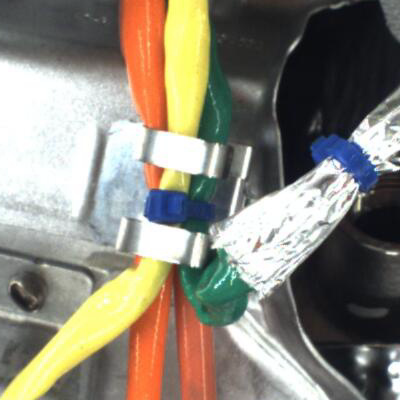
\includegraphics[width=\textwidth]{figures/good-engine-wiring-0000.png}
    \caption*{Good sample}
\end{minipage}
\hfill
\begin{minipage}{0.48\textwidth}
    \centering
    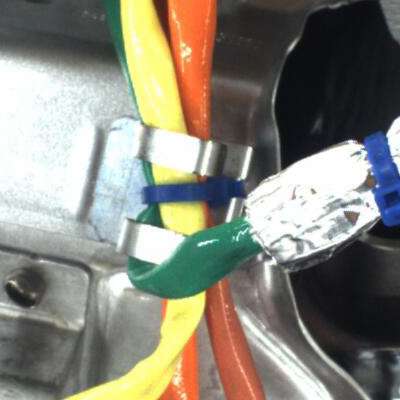
\includegraphics[width=\textwidth]{figures/defect-engine-wiring-obstruction-0000.png}
    \caption*{Defect sample}
\end{minipage}

\caption{Comparison between good and defect engine wiring samples.}
\label{fig:engine-wiring-comparison}
\end{figure}
\FloatBarrier

The count of test files is shown below:

\begin{table}[htbp]
    \centering
    \begin{tabular}{l r}
        \hline
        \textbf{Category} & \textbf{\# Test Files} \\
        \hline
        engine\_wiring    & 607 \\
        pipe\_clip        & 337 \\
        pipe\_staple      & 305 \\
        tank\_screw       & 413 \\
        underbody\_pipes  & 345 \\
        underbody\_screw  & 392 \\
        \hline
    \end{tabular}
    \caption{Number of test files per category in the AutoVI dataset.}
    \label{tab:test_files_per_category}
\end{table}

We also show below a split of the whole test dataset based on defect type:

\begin{table}[htbp]
    \centering
    \begin{tabular}{l r}
        \hline
        \textbf{Defect Type} & \textbf{\# Test Images} \\
        \hline
        good         & 1521 \\
        blue\_hoop    & 5 \\
        cardboard     & 5 \\
        fastening     & 277 \\
        multiple      & 34 \\
        obstruction   & 182 \\
        operator      & 4 \\
        unclipped     & 141 \\
        missing       & 230 \\
        \hline
    \end{tabular}
    \caption{Counts of good and defect types across the Test split.}
    \label{tab:defects_test_split}
\end{table}

In addition to the AutoVI dataset presented previously, we also evaluate our approach on three additional industrial visual inspection datasets: \textit{XFK3}, \textit{Pompe}, and \textit{Radiateur}.
These datasets follow a binary inspection paradigm, where parts are labeled as \textbf{OK} (non-defective) or \textbf{KO} (defective).

All datasets consist of high-resolution RGB images acquired in controlled industrial environments.
Training is performed primarily on OK samples, while KO samples are used for evaluation, in line with the anomaly detection setting.

\subsection{XFK3 Dataset}

The \textbf{XFK3} dataset contains images of a circular metallic component, where defects typically manifest as surface irregularities, contaminations, or structural anomalies.

The dataset is split into training and testing subsets, with a strong class imbalance typical for real-world quality inspection tasks.

\paragraph{Training Split}
\begin{itemize}
    \item OK: 1204 images
    \item KO: 19 images
\end{itemize}

\paragraph{Test Split}
\begin{itemize}
    \item OK: 134 images
    \item KO: 2 images
\end{itemize}

\begin{table}[htbp]
    \centering
    \begin{tabular}{l r r}
        \hline
        \textbf{Split} & \textbf{\# OK} & \textbf{\# KO} \\
        \hline
        Train & 1204 & 19 \\
        Test  & 134  & 2 \\
        \hline
    \end{tabular}
    \caption{Class distribution for the XFK3 dataset.}
    \label{tab:xfk3_distribution}
\end{table}

Figure~\ref{fig:xfk3_example} illustrates an example from the XFK3 dataset together with the corresponding explainability output generated by the PatchCore model.

\begin{figure}[htbp]
    \centering
    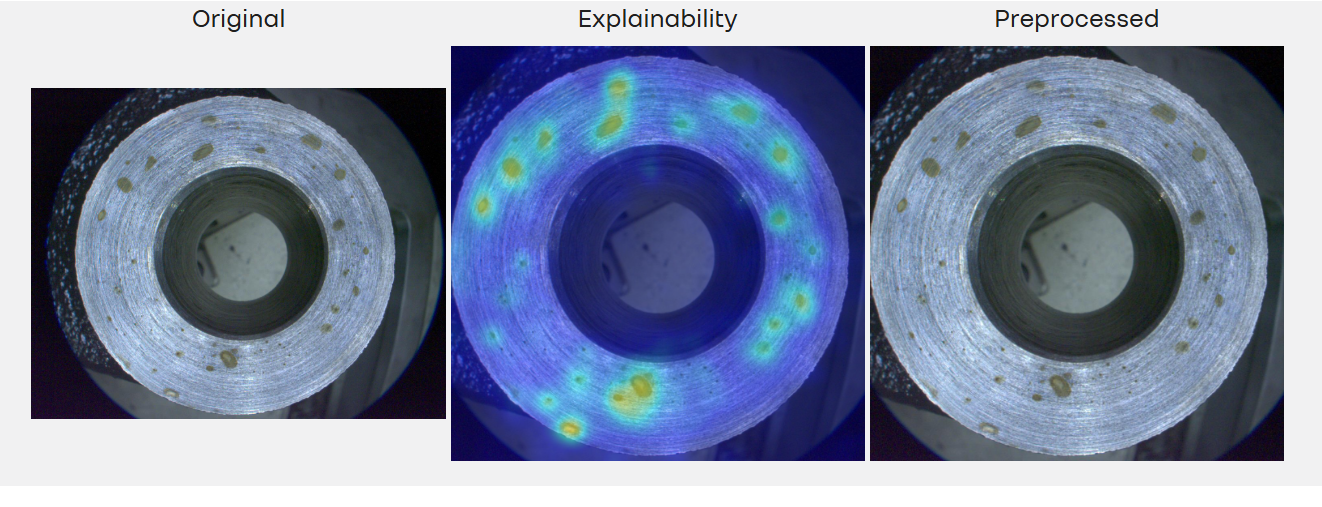
\includegraphics[width=0.9\textwidth]{figures/xfk3_explainability_example.png}
    \caption{Example XFK3 sample}
    \label{fig:xfk3_example}
\end{figure}
\FloatBarrier

\subsection{Pompe Dataset}

The \textbf{Pompe} dataset contains images of pump components inspected for manufacturing defects such as deformations, missing elements, or surface damage.

Unlike XFK3, this dataset includes an explicit validation split in addition to training and testing.

\paragraph{Training Split}
\begin{itemize}
    \item OK: 170 images
    \item KO: 30 images
\end{itemize}

\paragraph{Validation Split}
\begin{itemize}
    \item OK: 85 images
    \item KO: 15 images
\end{itemize}

\paragraph{Test Split}
\begin{itemize}
    \item OK: 28 images
    \item KO: 5 images
\end{itemize}

\begin{table}[htbp]
    \centering
    \begin{tabular}{l r r}
        \hline
        \textbf{Split} & \textbf{\# OK} & \textbf{\# KO} \\
        \hline
        Train & 170 & 30 \\
        Validation & 85 & 15 \\
        Test & 28 & 5 \\
        \hline
    \end{tabular}
    \caption{Class distribution for the Pompe dataset.}
    \label{tab:pompe_distribution}
\end{table}

Figure~\ref{fig:pompe_defect} presents a representative defective sample from the Pompe dataset.

\begin{figure}[htbp]
    \centering
    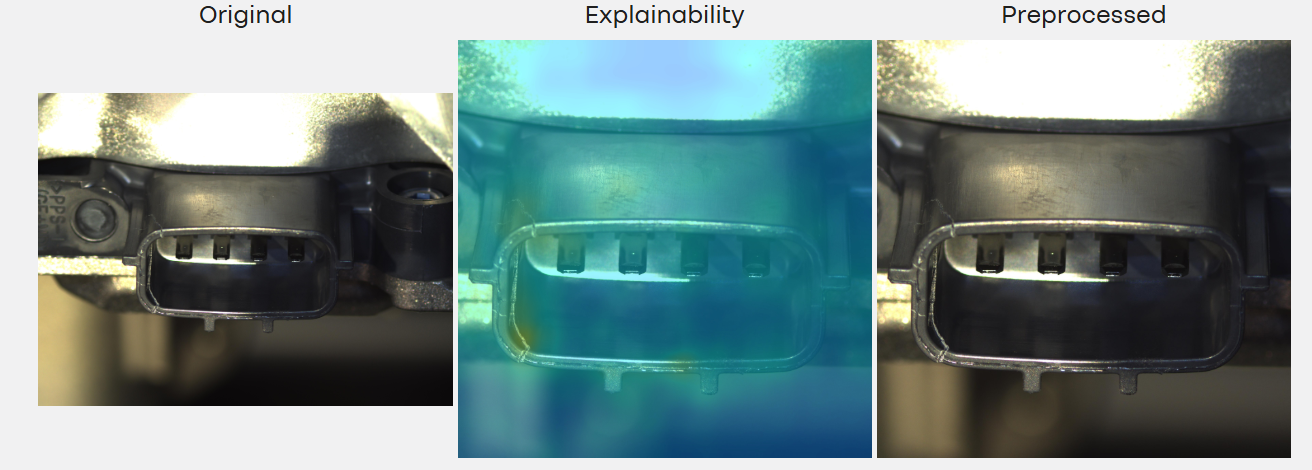
\includegraphics[width=0.75\textwidth]{figures/pompe_defect_example.png}
    \caption{Example of a defective sample from the Pompe dataset.}
    \label{fig:pompe_defect}
\end{figure}
\FloatBarrier

\subsection{Radiateur Dataset}

The \textbf{Radiateur} dataset consists of images of radiator assemblies, where defects may include structural misalignments, missing clips, or assembly errors.

Similarly to the Pompe dataset, Radiateur includes a dedicated validation split.

\paragraph{Training Split}
\begin{itemize}
    \item OK: 197 images
    \item KO: 26 images
\end{itemize}

\paragraph{Validation Split}
\begin{itemize}
    \item OK: 98 images
    \item KO: 14 images
\end{itemize}

\paragraph{Test Split}
\begin{itemize}
    \item OK: 34 images
    \item KO: 4 images
\end{itemize}

\begin{table}[htbp]
    \centering
    \begin{tabular}{l r r}
        \hline
        \textbf{Split} & \textbf{\# OK} & \textbf{\# KO} \\
        \hline
        Train & 197 & 26 \\
        Validation & 98 & 14 \\
        Test & 34 & 4 \\
        \hline
    \end{tabular}
    \caption{Class distribution for the Radiateur dataset.}
    \label{tab:radiateur_distribution}
\end{table}

Figure~\ref{fig:radiateur_example} shows a Radiateur sample together with its preprocessing and explainability output.

\begin{figure}[htbp]
    \centering
    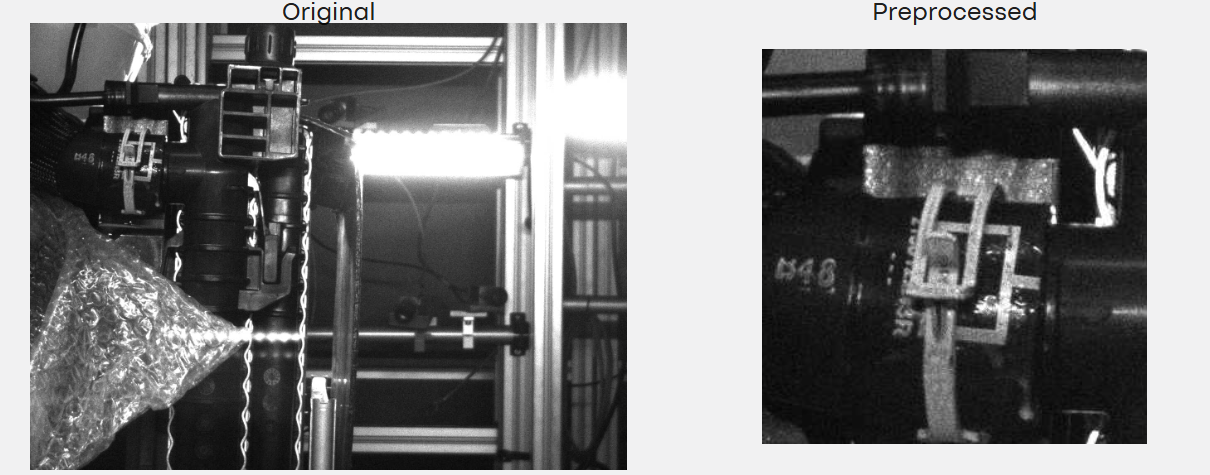
\includegraphics[width=0.9\textwidth]{figures/radiateur_explainability_example.png}
    \caption{Example Radiateur sample}
    \label{fig:radiateur_example}
\end{figure}
\FloatBarrier

\section{Baseline Model Architecture}

For our baseline anomaly detection model, we employ PatchCore \citep{Roth2022TotalRecall}, a memory-based approach that achieves state-of-the-art performance on industrial anomaly detection tasks without requiring defect samples during training.

\subsection{PatchCore Overview}

PatchCore operates by extracting features from normal (non-defective) images using a pre-trained convolutional neural network backbone. Rather than training a classifier, PatchCore builds a memory bank of representative patch-level features from the training set. During inference, anomalies are detected by measuring the deviation of test image features from this learned distribution of normal patterns.

The key components of our PatchCore implementation are:

\begin{itemize}
    \item \textbf{Feature Extraction}: We use a pre-trained Wide ResNet-50 backbone to extract multi-scale features at intermediate layers (specifically layers 2 and 3). These features capture both low-level textures and high-level semantic information.

    \item \textbf{Memory Bank Construction}: From the extracted training features, we construct a compact memory bank using coreset subsampling. This reduces the computational burden while maintaining representative coverage of the normal feature space.

    \item \textbf{Anomaly Scoring}: At test time, for each patch in the input image, we compute its distance to the nearest neighbor in the memory bank. High distances indicate anomalous regions.
\end{itemize}

\subsection{Implementation Details}

Our implementation uses the following configuration:
\begin{itemize}
    \item Input image size: $224 \times 224$ pixels
    \item Batch size: 32
    \item Coreset sampling ratio: 10\% (random sampling for baseline)
    \item Feature dimension: 1536 (concatenated from two ResNet layers)
    \item Device: CUDA-enabled GPU
\end{itemize}

For each of the six AutoVI categories, we train a separate PatchCore model, as each category exhibits distinct visual characteristics and defect patterns.

\paragraph*{Justification of choosing coreset ratio}

The 10\% coreset sampling ratio is in line with the original PatchCore 
recommendation~\citep{Roth2022TotalRecall}, which showed that keeping 
a tenth of the full patch feature set gives enough coverage of the 
nominal distribution while keeping memory and nearest-neighbour search 
manageable during inference. At this ratio, the largest category 
(\texttt{underbody\_screw}, 373 training images) yields approximately 
$3 \times 10^4$ patches before subsampling --- a bank size where 
k-center selection remains feasible within the chunked implementation 
(\texttt{coreset\_chunk\_size} $= 8192$).

Greedy k-center selection requires repeated distance computations 
between candidate features and the current selected set. To avoid 
materialising the full $N \times N$ distance matrix, the implementation 
processes features in chunks of 8192 rows at a time, updating a 
running minimum-distance vector. This value balances GPU memory 
pressure against iteration overhead, consistent with typical 
$L_2$-distance batch sizes used in PatchCore-style retrieval pipelines.

\subsection{Centralized Learning Results}

We first establish baseline performance by training PatchCore models in a centralized manner, where all training data for each category is available to a single model. Table \ref{tab:centralized_results_random} presents the performance metrics across all six categories using random coreset sampling.

\begin{table}[htbp]
    \centering
    \begin{tabular}{l c c c c}
        \hline
        \textbf{Category} & \textbf{Image AUROC} & \textbf{Pixel AUROC} & \textbf{Image AP} & \textbf{Pixel AP} \\
        \hline
        engine\_wiring     & 0.548 & 0.857 & 0.596 & 0.014 \\
        pipe\_clip         & 0.511 & 0.808 & 0.425 & 0.016 \\
        pipe\_staple       & 0.587 & 0.793 & 0.465 & 0.033 \\
        tank\_screw        & 0.473 & 0.817 & 0.216 & 0.004 \\
        underbody\_pipes   & 0.829 & 0.877 & 0.743 & 0.244 \\
        underbody\_screw   & 0.605 & 0.988 & 0.058 & 0.014 \\
        \hline
        \textbf{Average}   & 0.592 & 0.857 & 0.417 & 0.054 \\
        \hline
    \end{tabular}
    \caption{Centralized PatchCore with random coreset performance on AutoVI dataset. AUROC = Area Under ROC Curve, AP = Average Precision.}
    \label{tab:centralized_results_random}
\end{table}

The centralized models using random sampling achieve strong pixel-level AUROC scores (average 0.857), indicating good localization of defects. Image-level AUROC is more modest (average 0.592), reflecting the challenge of binary classification on this industrial dataset. Notably, underbody\_screw achieves exceptional pixel-level AUROC of 0.988, while underbody\_pipes shows the best image-level performance at 0.829.
\\

Next, we employ K-center coreset sampling, which greedily selects the most diverse subset of features by repeatedly choosing the point farthest from the current selected set, approximating a minimal-cover representative set.

\begin{table}[htbp]
      \centering
      \begin{tabular}{l c c c c}
          \hline
          \textbf{Category} & \textbf{Image AUROC} & \textbf{Pixel AUROC} & \textbf{Image AP} & \textbf{Pixel AP} \\
          \hline
          engine\_wiring     & 0.662 & 0.842 & 0.650 & 0.020 \\
          pipe\_clip         & 0.521 & 0.822 & 0.422 & 0.028 \\
          pipe\_staple       & 0.469 & 0.830 & 0.383 & 0.077 \\
          tank\_screw        & 0.570 & 0.776 & 0.241 & 0.015 \\
          underbody\_pipes   & 0.952 & 0.863 & 0.914 & 0.346 \\
          underbody\_screw   & 0.951 & 0.990 & 0.341 & 0.260 \\
          \hline
          \textbf{Average}   & 0.687 & 0.854 & 0.492 & 0.124 \\
          \hline
      \end{tabular}
      \caption{Centralized PatchCore performance with kcenter coreset on AutoVI dataset. AUROC = Area Under ROC Curve, AP = Average Precision.}
      \label{tab:centralized_results}
  \end{table}

On average, using kcenter coreset sampling improves Image AUROC (+0.095) and Image AP (+0.075), while Pixel AUROC is essentially flat ($-0.003$) and Pixel AP improves (+0.070). The average masks huge per-category variance. The biggest gains are in the underbody categories (both image- and pixel-level metrics jump notably), while pipe\_staple's image AUROC drops relative to the previous ablation. Overall, the updated results shift toward stronger image-level discrimination without a clear change in pixel AUROC.

In the figures below we can observe the difference in a visual manner.
\begin{figure}[htbp]
    \centering
    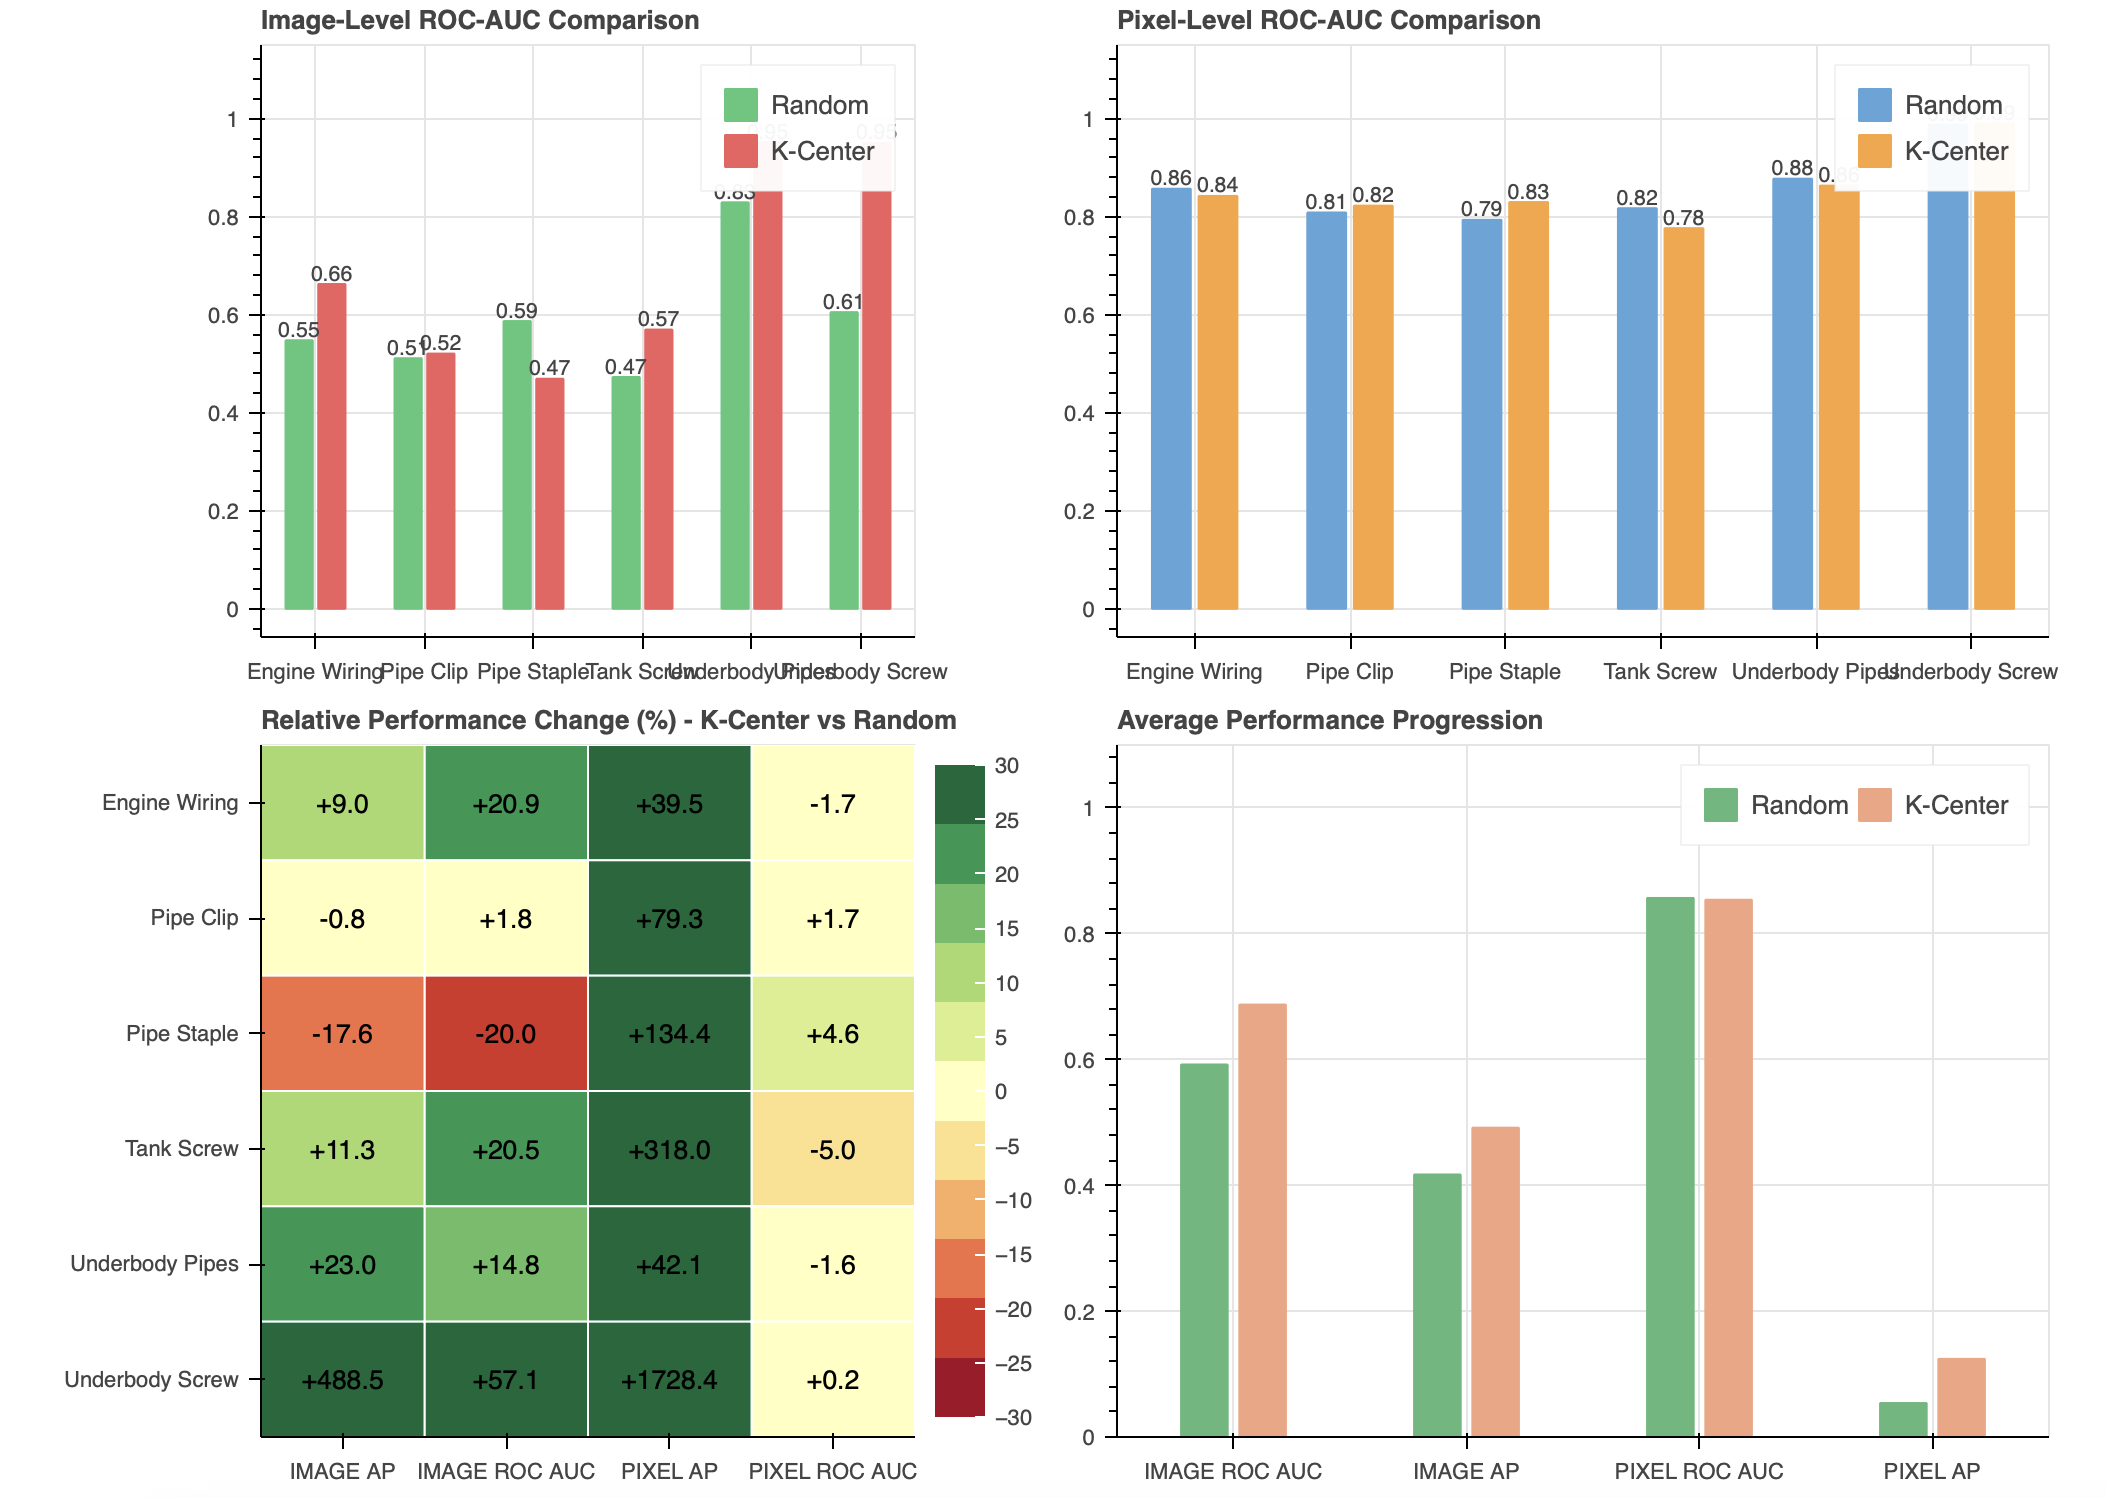
\includegraphics[width=\textwidth]{figures/comparison-central-random-kcenter.png}
    \caption{Comprehensive performance comparison showing: (top-left) image-level AUROC, (top-right) pixel-level AUROC, (bottom-left) performance degradation heatmap, (bottom-right) average metrics across all categories.}
    \label{fig:comparisoncrk002}
\end{figure}
\FloatBarrier

\begin{figure}[htbp]
    \centering
    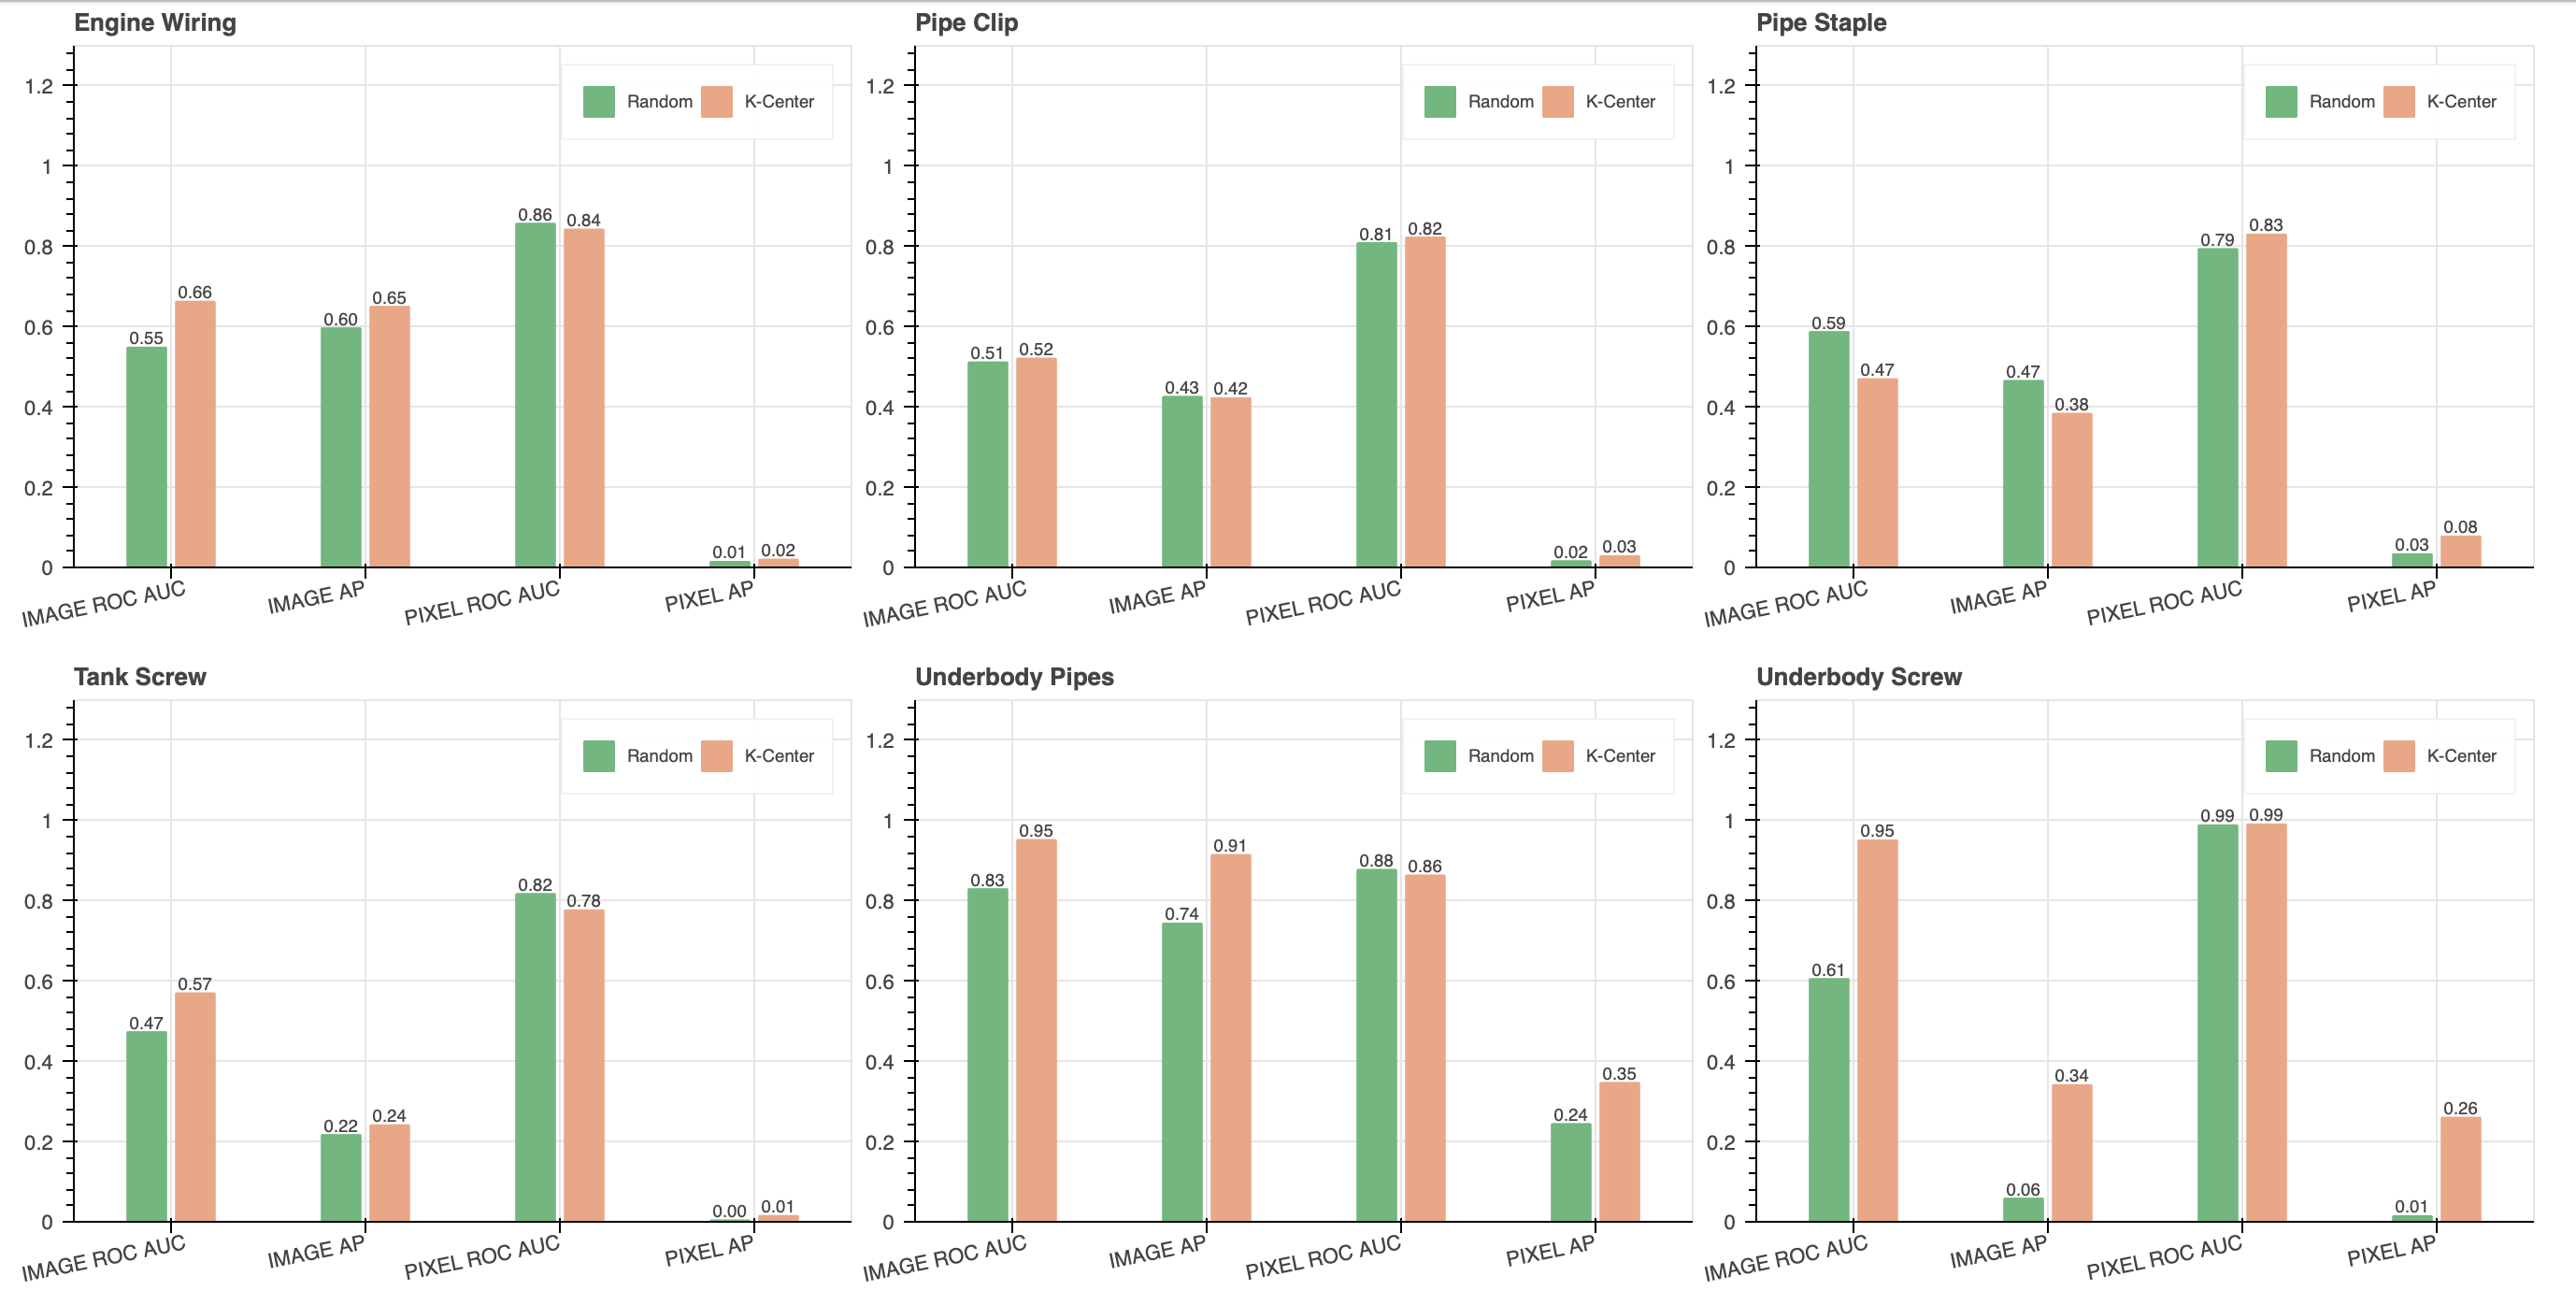
\includegraphics[width=\textwidth]{figures/comparison-central-random-kcenter-detailed.png}
    \caption{Detailed per-category comparison of all four evaluation metrics (Image AUROC, Pixel AUROC, Image AP, Pixel AP) between random and K-Center coreset sampling strategies.}
    \label{fig:detailed_comparisoncrk002}
\end{figure}
\FloatBarrier

\section{Federated Setup}

To investigate privacy-preserving anomaly detection, we implement a custom federated learning framework. Our setup simulates a realistic scenario where different production lines or facilities possess data for different product categories.

\subsection{Architecture}

Our federated implementation consists of:

\begin{itemize}
    \item \textbf{Server}: Coordinates the federated training process, aggregates memory banks from clients, and distributes the global model. The server uses a custom FedAvg strategy adapted for memory bank aggregation rather than traditional model parameter averaging.

    \item \textbf{Clients}: Each client represents a production facility with access to training data for a subset of categories. Clients extract features locally, build category-specific memory banks, and share these with the server.
\end{itemize}

\subsection{Data Partitioning}

We simulate a non-IID (non-independent and identically distributed) data split across three clients:

\begin{itemize}
    \item \textbf{Client 1}: engine\_wiring, pipe\_clip
    \item \textbf{Client 2}: pipe\_staple, tank\_screw
    \item \textbf{Client 3}: underbody\_pipes, underbody\_screw
\end{itemize}

This partitioning reflects a realistic industrial scenario where different production facilities specialize in different components.

\subsection{Aggregation Method}

Unlike traditional federated learning that averages model weights, our approach aggregates memory banks:

\begin{enumerate}
    \item Each client extracts features from local training data and constructs category-specific memory banks
    \item Clients send their memory banks to the server
    \item The server concatenates all memory banks for each category
    \item To limit computational cost, the server applies random sampling to cap each category's memory bank at 50,000 features
    \item The aggregated global memory banks are distributed back to clients for evaluation
\end{enumerate}

This process is repeated for 3 federated rounds.

\subsection{Implementation Details}

Key configuration parameters for the federated setup:

\begin{itemize}
    \item Number of clients: 3
    \item Number of federated rounds: 3
    \item Memory bank size limit: 50,000 features per category
    \item Aggregation method: Concatenation + random sampling
    \item Communication protocol: custom framework based on pickle RPC
\end{itemize}

We implement a custom federated learning mechanism based on pickle RPC. We chose this over readily available frameworks such as Flower because their strict synchronous client requirements are difficult to implement in practice, particularly given hardware availability constraints. Our custom framework allowed asynchronous operation and separate upload and eval modes for clients. In the upload mode the client builds local memory banks and uploads them to the server. Once all clients have completed building their memory banks, the server will concatenate category banks and apply k-center coreset. In the eval mode the clients will download global banks into the trainer and compute the metrics.
	\\
\begin{adjustbox}{max width=\textwidth, max height=0.32\textheight, keepaspectratio, center}
    \begin{sequencediagram}

      \tikzstyle{every node}=[font=\fontsize{8.5}{9}\selectfont]

      \tikzstyle{inststyle}+=[minimum height=0.6cm, minimum width=3.5cm, font=\fontsize{8}{9}\selectfont]

      \newthread{client}{Client}
      \newthread{server}{Server}

      \begin{callself}{client}{fit(category) x N}{memory\_banks, patch\_shapes}
      \end{callself}

      \begin{call}{client}{RPC upload (pickle + 8B len)}{server}{ok}
      \end{call}

      \begin{callself}{server}{aggregate (concat + k-center)}{global\_banks}
      \end{callself}

      \begin{call}{client}{RPC download (pickle + 8B len)}{server}{global\_banks, patch\_shapes}
      \end{call}

      \begin{callself}{client}{evaluate(category) x N}{metrics}
      \end{callself}

      \begin{callself}{client}{write client\_X\_metrics.json}{done}
      \end{callself}

    \end{sequencediagram}
  \end{adjustbox}

As aggregation strategy we now concatenate and applies k-center greedy coreset selection with configurable maximum server samples and chunk sizes. We also implemented deterministic train splits.


The two figures below visualize the comparisons between the federated implementation versus the baseline centralized training loop, all using kcenter for coreset sampling.

\begin{figure}[htbp]
    \centering
    
\includegraphics[width=\textwidth]{figures/comparison002.png}
    \caption{Comprehensive performance comparison showing: (top-left) image-level AUROC, (top-right) pixel-level AUROC, (bottom-left) performance degradation heatmap, (bottom-right) average metrics across all categories.}
    \label{fig:comparison002}
\end{figure}
\FloatBarrier

\begin{figure}[htbp]
    \centering
    
\includegraphics[width=\textwidth]{figures/detailed-comparison002.png}
    \caption{Detailed per-category comparison of all four evaluation metrics (Image AUROC, Pixel AUROC, Image AP, Pixel AP) between centralized and federated approaches.}
    \label{fig:detailed_comparison002}
\end{figure}
\FloatBarrier

In four out of six categories, federated training with k-center aggregation does as well or better than centralized training on image-level ROC AUC. The biggest absolute gains are in \texttt{underbody\_pipes} (0.95 → 1.00) and \texttt{underbody\_screw} (0.95 → 0.99). It may seem strange, but putting data on three non-IID clients does not make it harder to tell the difference between normal and abnormal data. In fact, it can make it easier. One possible reason is that server-side k-center aggregation across concatenated client banks creates a more diverse coreset than any single client could make on its own, which is like adding more data to the feature space. Pixel-level ROC AUC stays stable across all categories $\Delta \leq 0.02$, which shows that spatial localization works well even when the data is split up across different servers. 

\section {Trust-Enhancing Mechanisms}

As discussed in \citep{liu2021trustworthyaicomputationalperspective} there are six crucial dimensions to AI trustworthiness: (i) Safety \& Robustness, (ii) Non-discrimination \& Fairness, (iii) Explainability, (iv) Privacy, (v) Accountability \& Auditability, and (vi) Environmental Well-Being. To study the effects of trustworthiness on automotive anomaly detection, we pick four dimensions that we implement and measure in our pipeline: Privacy, Fairness, Interpretability and Robustness.

\subsection{Privacy}
\subsubsection{Differential Privacy}



First introduced by \citep{Dwork2006Calibrating} we implement differential privacy at the client before sending features to the server, so each client's contribution is bounded and noisy.
\begin{itemize}
  \item \textbf{Where it happens:} after the client builds a per-category memory bank (coreset), but before upload.
  \item \textbf{Clip:} for each category, clip each feature vector to a fixed $L_2$ norm $C$ (bounds sensitivity).
  \item \textbf{Noise:} add Gaussian noise calibrated to $C$, dataset size, and target $(\varepsilon, \delta)$ so the uploaded coreset is DP.
  \item \textbf{Guarantee:} the server only ever sees a privatized coreset; privacy depends on the DP mechanism, not trust in the server.
  \item \textbf{Accounting:} track the per-round and total privacy loss $(\varepsilon, \delta)$ with a standard accountant (e.g., RDP or moments accountant) and log the cumulative budget for the run.
\end{itemize}
In short: we constrain and perturb each client's memory bank so the transmission itself is differentially private, and report the total privacy cost for the training session.

Introducing differential privacy decreases our scores almost to the level of centralized training.

\begin{figure}[htbp]
    \centering
    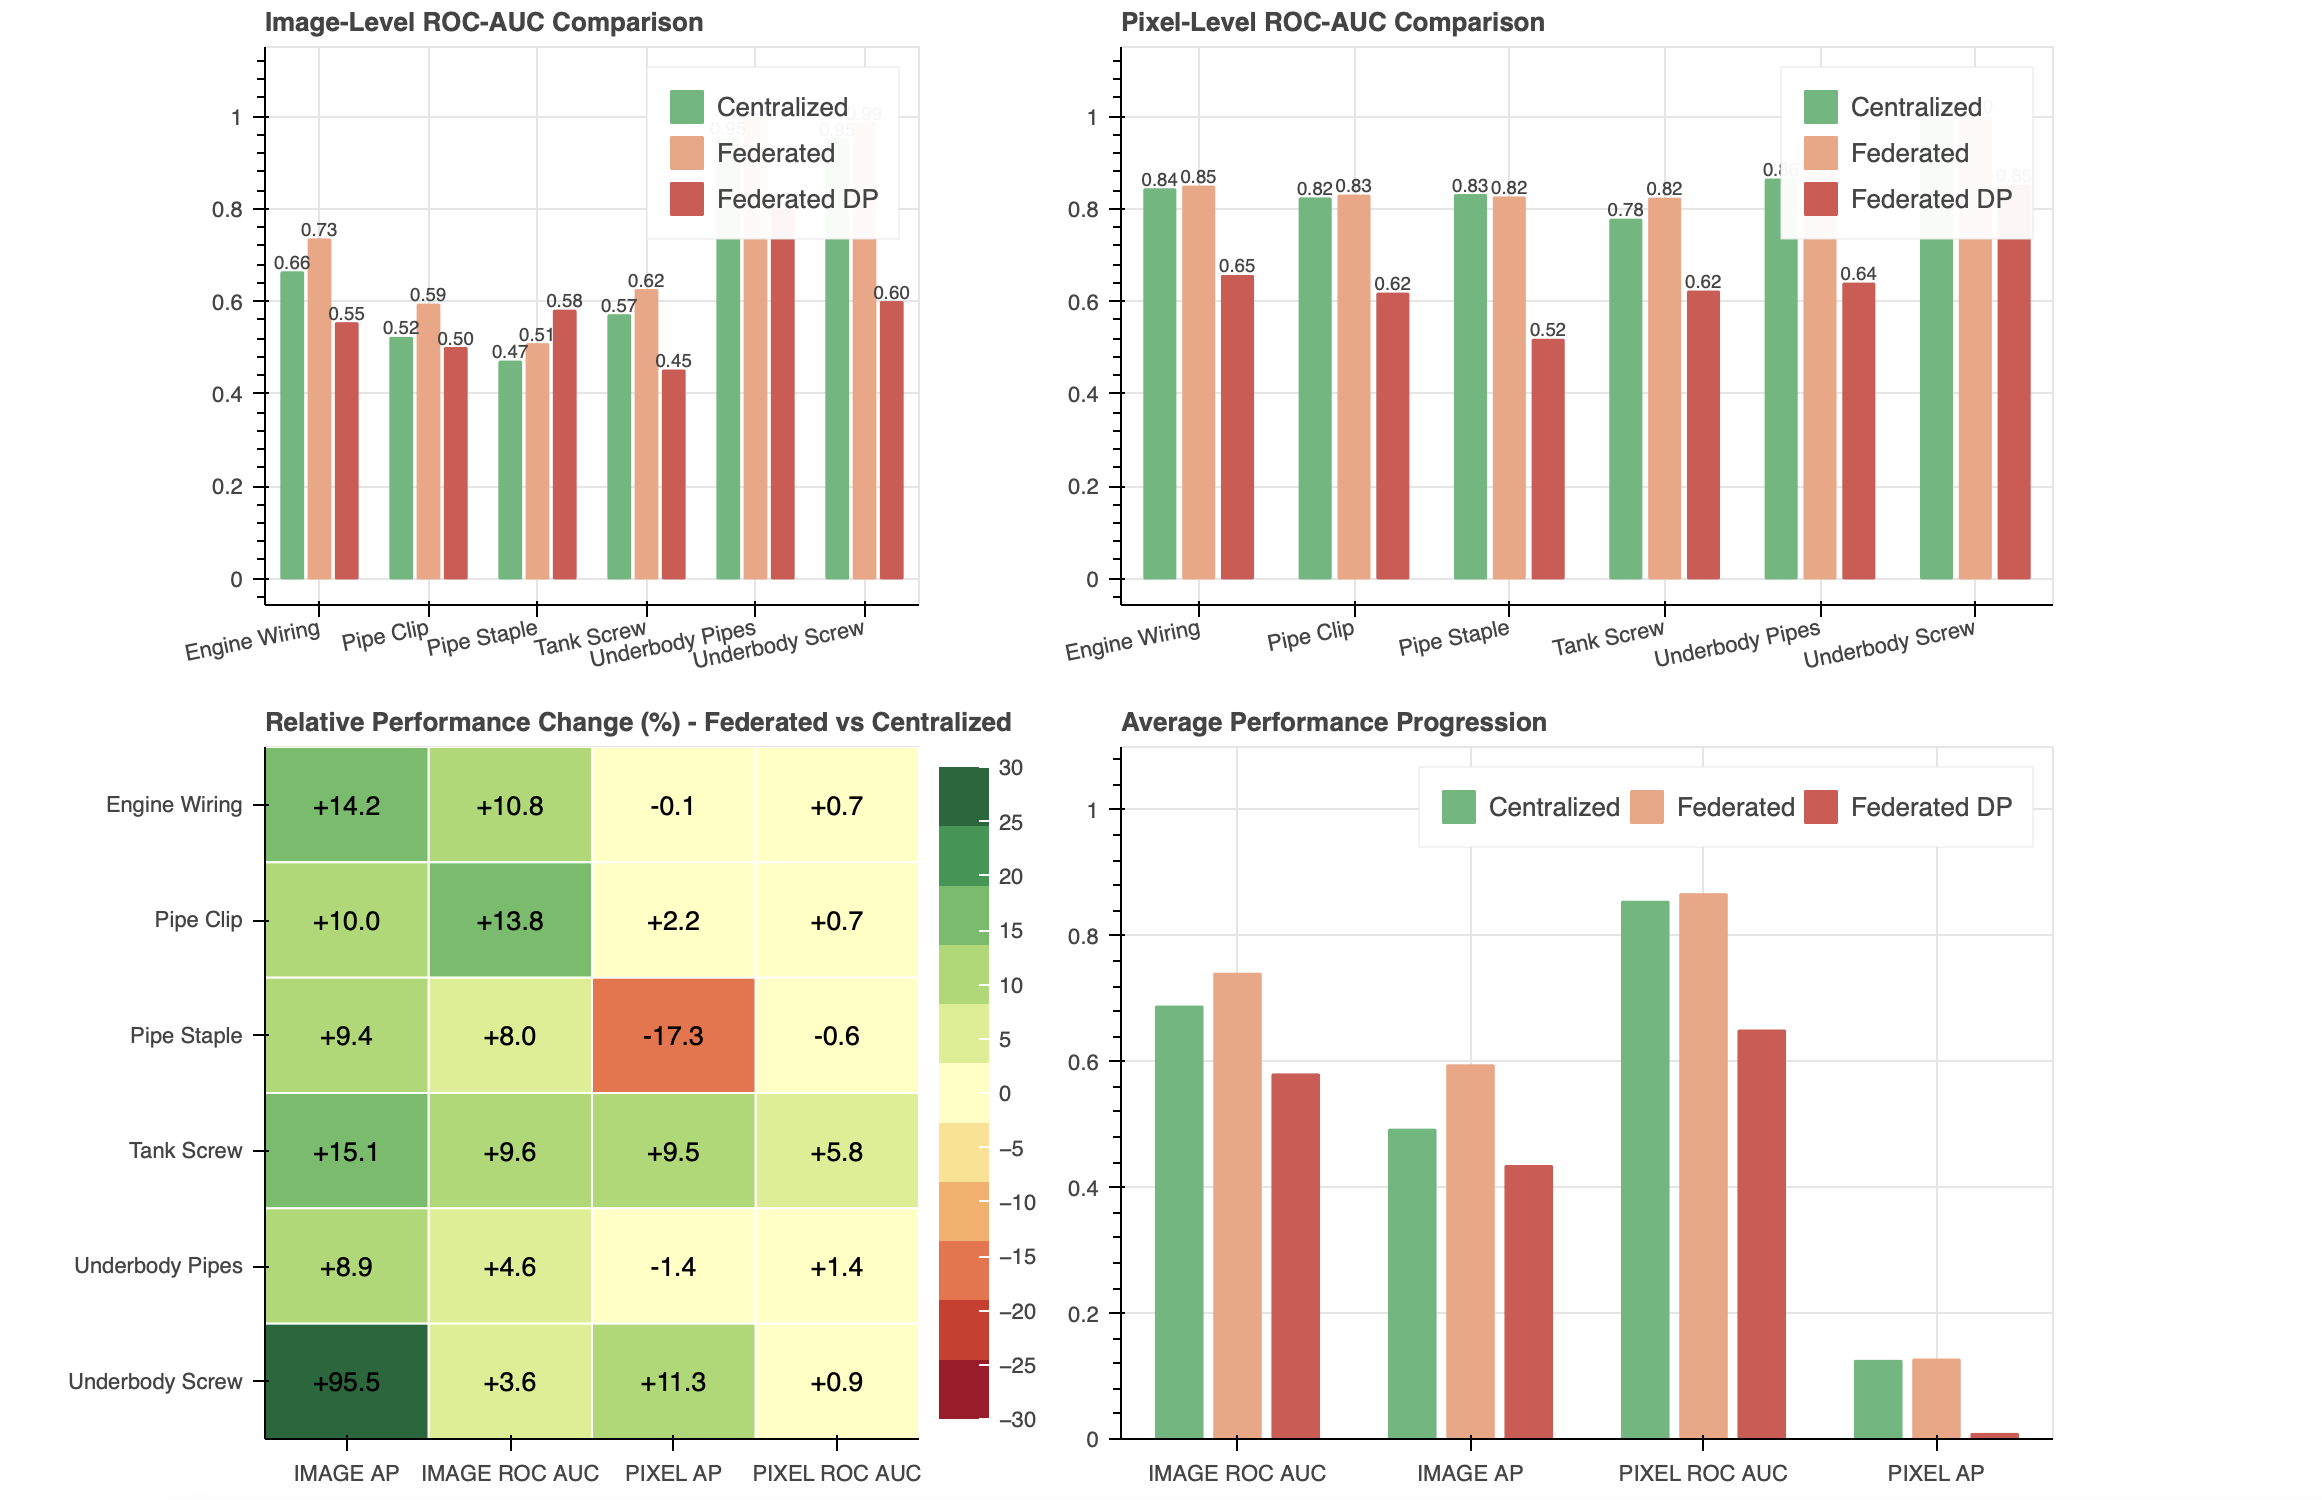
\includegraphics[width=\textwidth]{figures/comparison003.png}
    \caption{Comprehensive performance comparison showing: (top-left) image-level AUROC, (top-right) pixel-level AUROC, (bottom-left) performance degradation heatmap, (bottom-right) average metrics across all categories.}
    \label{fig:comparison003}
\end{figure}
\FloatBarrier

\begin{figure}[htbp]
    \centering
    
\includegraphics[width=\textwidth]{figures/detailed-comparison003.png}
    \caption{Detailed per-category comparison of all four evaluation metrics (Image AUROC, Pixel AUROC, Image AP, Pixel AP) between centralized and federated approaches.}
    \label{fig:detailed_comparison003}
\end{figure}
\FloatBarrier

When we add differential privacy to client uploads, both image- and pixel-level metrics drop significantly compared to the non-private federated baseline. The average Image ROC AUC drops from 0.74 to 0.58, and it only partially recovers to centralized levels (0.69). The degradation isn't the same for all categories. For example, \texttt{underbody\_pipes} still has a good discrimination rate of 0.80 compared to 1.00 without DP, but \texttt{tank\_screw} drops to 0.45, which is lower than the centralized baseline of 0.57. Pixel ROC AUC drops from an average of 0.87 (federated) to 0.65 (federated-DP), and \texttt{pipe\_staple} drops to 0.52. The difference between image-level and pixel-level degradation suggests that the Gaussian noise added at the feature level breaks up fine-grained spatial structure more than coarse discriminative signal. At $\varepsilon \approx 1.45$, the privacy-utility trade-off is very aggressive. The budget is tight enough to provide good protection, but the cost would probably be too high for production deployment without more noise calibration.

\paragraph*{Justification for choosing DP Parameters}

Using the standard Gaussian mechanism formula, the noise scale is directly derived from the target privacy budget: \begin{equation} \sigma = \frac{\sqrt{2 \ln(1.25 / \delta)}}{\varepsilon} \end{equation} with the per-feature noise standard deviation set to $\sigma \cdot C$, where $C$ is the $L_2$ clipping threshold. For datasets of this size, we set $\delta = 10^{-5}$, which is a standard choice. For all six categories, where $N \leq 373$, the rule of thumb $\delta \ll 1/N$ is satisfied. 
In order to ensure that clipping eliminates actual outliers rather than systematically shrinking all vectors, the clipping norm $C = 1.0$ is selected to match the typical $L_2$ magnitude of Wide ResNet-50 intermediate features following ImageNet normalization. 
To achieve a strong privacy guarantee, the target $\varepsilon = 1.45$ is chosen; values below $2.0$ are typically regarded as tight for sensitive industrial data. According to the performance results in Section~\ref{sec:rdp_results}, the Gaussian mechanism produces $\sigma \approx 4.84$ under these conditions, which means the injected noise is almost five times the magnitude of the clipped signal. This is a purposeful trade-off that prioritizes privacy over utility.


\subsubsection{Renyi Differential Privacy}
\label{sec:rdp_results}
Introduced by \citep{Mironov_2017} Rényi Differential Privacy (RDP) is a generalization of differential privacy that provides a more mathematically tractable way to analyze the composition of private mechanisms, particularly for iterative algorithms.
 \\
A randomized mechanism $\mathcal{M}$ satisfies $(\alpha, \epsilon)$-RDP if for any two adjacent datasets $D, D'$ (differing in a single element), the Rényi divergence of order $\alpha$ between their output distributions is bounded by
      $\epsilon$:
   \begin{equation}
   D_\alpha(\mathcal{M}(D) || \mathcal{M}(D')) \le \epsilon
   \end{equation}
where the Rényi divergence of order $\alpha > 1$ between distributions $P$ and $Q$ is defined as:
 \begin{equation}
     D_\alpha(P || Q) = \frac{1}{\alpha - 1} \ln \mathbb{E}_{x \sim Q} \left[ \left( \frac{P(x)}{Q(x)} \right)^\alpha \right]
 \end{equation}
 \\
 RDP is a stronger definition than $(\epsilon, \delta)$-DP. If a mechanism satisfies $(\alpha, \epsilon)$-RDP, then it also satisfies $\left(\epsilon + \frac{\ln(1/\delta)}{\alpha-1}, \delta\right)$-DP for any $\delta \in (0, 1)$. This conversion allows researchers to track privacy loss in the RDP domain and translate the final bound back to the standard DP language.

\paragraph*{Justification for choosing RDP orders}

The tightest $(\varepsilon, \delta)$-DP bound is obtained by selecting the order that minimizes over a grid of Renyi orders $\alpha \in \{1.25,\ 1.5,\ 2,\ 3,\ 4,\ 5,\ 8,\ 10,\ 16,\ 32,\ 64,\ 128\}$. Here, $T$ denotes the number of composition steps, i.e., the number of categories released per client. The accountant chooses $\alpha = 16$ as the optimal order under the experimental configuration ($\sigma \approx 4.84$, $T = 2$, $\delta = 10^{-5}$), yielding a total $\varepsilon \approx 1.45$. The grid ensures that the minimum is not overlooked at either extreme by covering both low orders, where the divergence term predominates, and high orders, where the composition term predominates.
 
 \paragraph*{Key Properties}
\begin{itemize}
	\item \textbf{Composition:} If $\mathcal{M}_1$ satisfies $(\alpha, \epsilon_1)$-RDP and $\mathcal{M}_2$ satisfies $(\alpha, \epsilon_2)$-RDP, then their composition satisfies $(\alpha, \epsilon_1 + \epsilon_2)$-RDP. This linear composition is significantly tighter than the "Advanced Composition" theorem used in standard DP.
	\item \textbf{Gaussian Mechanism:} For a function $f$ with $L_2$-sensitivity $\Delta f$, the Gaussian mechanism $\mathcal{M}(D) = f(D) + \mathcal{N}(0, \sigma^2 I)$ satisfies $(\alpha, \alpha \Delta f^2 / 2\sigma^2)$-RDP.
 \end{itemize}

\begin{figure}[htbp]
    \centering
    
\includegraphics[width=\textwidth]{figures/comparison004.png}
    \caption{Comprehensive performance comparison showing: (top-left) image-level AUROC, (top-right) pixel-level AUROC, (bottom) average metrics across all categories.}
    \label{fig:comparison004}
\end{figure}
\FloatBarrier

\begin{figure}[htbp]
    \centering
    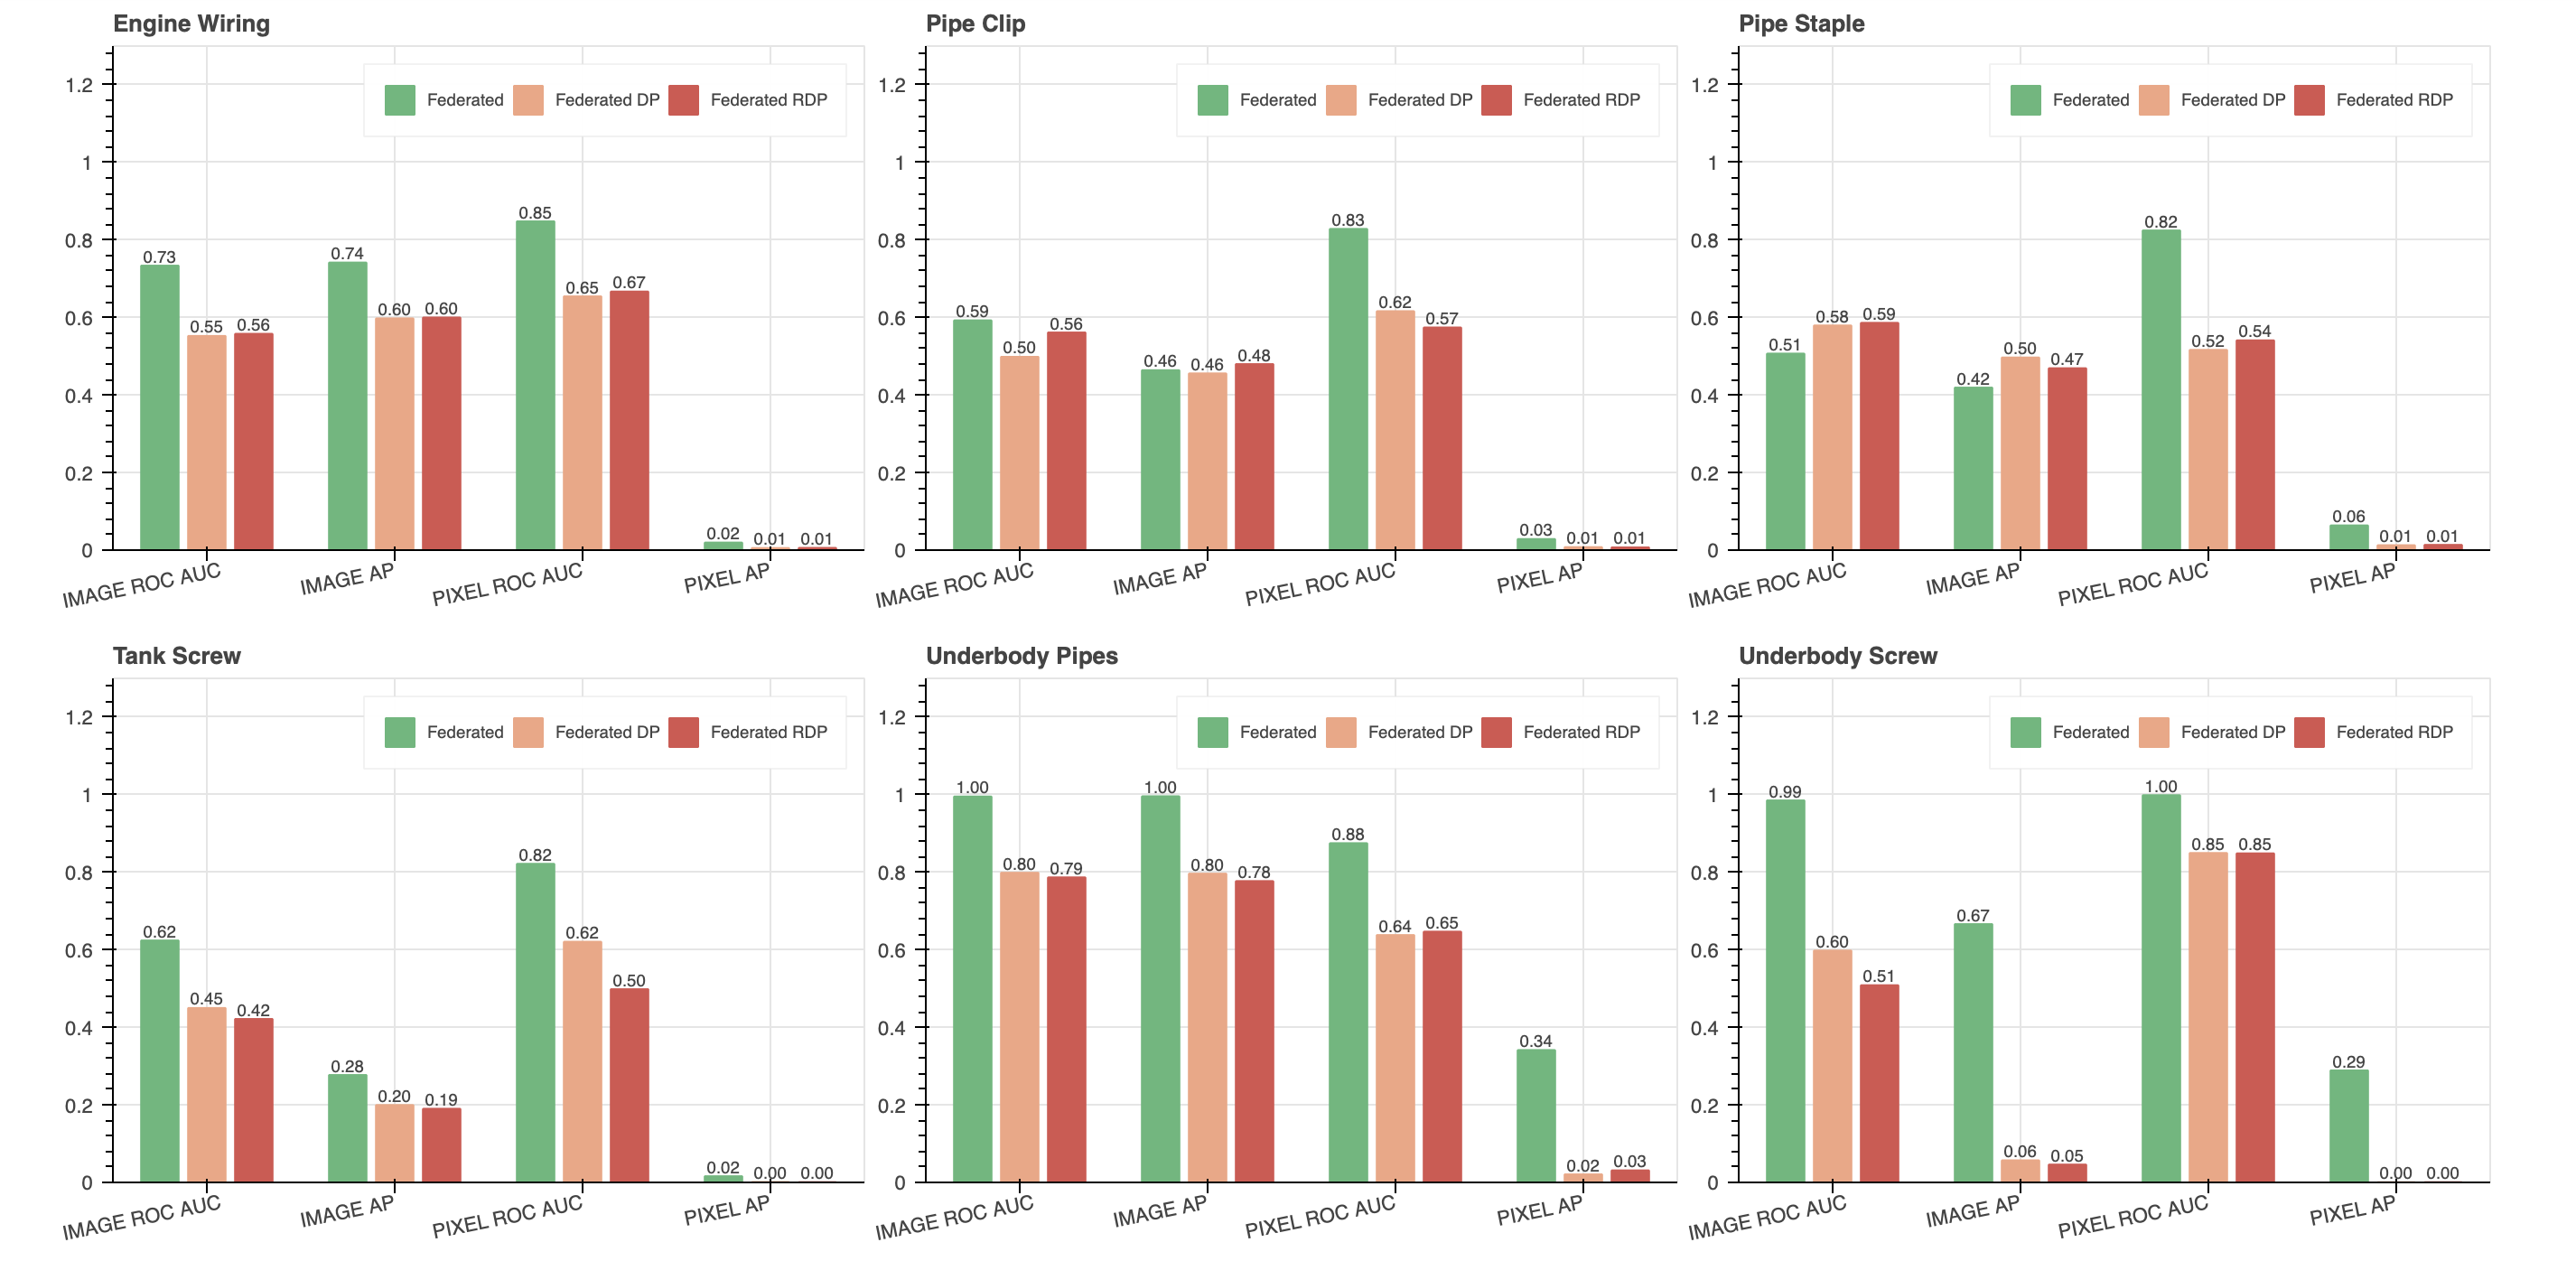
\includegraphics[width=\textwidth]{figures/detailed-comparison004.png}
    \caption{Detailed per-category comparison of all four evaluation metrics (Image AUROC, Pixel AUROC, Image AP, Pixel AP) between centralized and federated approaches.}
    \label{fig:detailed_comparison004}
\end{figure}
\FloatBarrier

Standard DP and RDP yield comparable utility outcomes, with RDP exhibiting a marginally inferior image-level AUC on average (0.57 versus 0.58), yet a slightly superior pixel-level ROC AUC in specific categories (e.g., \texttt{engine\_wiring}: 0.67 versus 0.65, \texttt{pipe\_staple}: 0.54 versus 0.52). The practical distinction between the two mechanisms is minimal given the selected parameterization. The primary theoretical advantage of RDP—stricter composition bounds—does not yield a quantifiable utility increase in this context, as the principal expense is the noise multiplier $\sigma \approx 4.84$, rather than composition across rounds. Both versions fail on \texttt{tank\_screw}, where the AUC for RDP image AUROC drops to 0.42, which is lower than random chance. This means that the discriminative features in this category are mostly found in a low-amplitude subspace that is more affected by high-variance Gaussian perturbations. Pixel AP drops to almost zero in all categories when either DP variant is used. This means that spatial localization doesn't really work at this privacy budget.

The results indicate a scenario with strong privacy guarantees but significantly degraded utility (anomaly detection performance).
The use of Differential Privacy (DP) with a high noise level has severely impacted the model's ability to distinguish between normal and anomalous images in most categories.

Privacy analysis
\begin{itemize}
    \item Privacy Budget ($\varepsilon$): $\approx 1.45$ (at $\delta = 10^{-5}$).\\
    \hspace*{1.5em}This is a tight/strong privacy budget. Values below 2.0 are generally considered excellent for sensitive data.
    \item Noise Multiplier ($\sigma$): $\approx 4.84$.\\
    \hspace*{1.5em}This is a very high amount of noise. For context, typical training runs might use $\sigma \approx 1.0$ to $1.5$. A value of nearly 5 means the noise added to the gradients/updates is roughly 5 times the magnitude of the clipped signal itself.
    \item Rényi Order ($\alpha$): $16.0$.\\
    \hspace*{1.5em}The accountant found that $\alpha = 16$ provided the tightest bound for this specific noise and step count.
\end{itemize}

Utility analysis:
\begin{itemize}
    \item Good performance:
    \begin{itemize}
        \item Underbody Pipes (Client 3): ROC AUC $\approx 0.79$.
        This category remained relatively robust to the noise, maintaining decent detection capability.
    \end{itemize}

    \item Poor performance (near random):
    \begin{itemize}
        \item Engine Wiring (Client 1): ROC AUC $\approx 0.56$.
        \item Pipe Clip (Client 1): ROC AUC $\approx 0.56$.
        \item Pipe Staple (Client 2): ROC AUC $\approx 0.59$.
    \end{itemize}

    \item Failure cases (worse than random):
    \begin{itemize}
        \item Tank Screw (Client 2): ROC AUC $\approx 0.42$.
        The noise likely overwhelmed the subtle features of this category, flipping the decision boundary (a score $<0.5$ suggests the model is effectively inverted or confused).
        \item Underbody Screw (Client 3): ROC AUC $\approx 0.51$.
    \end{itemize}
\end{itemize}

Conclusion:
The experiment prioritized privacy over utility. The high noise ($\sigma \approx 4.84$) ensured the epsilon remained low ($\approx 1.45$) despite the composition of mechanisms, but it rendered the model ineffective for finer‑grained anomalies (screws, wiring).

\subsection{Fairness}

To address potential bias in federated learning scenarios where clients possess imbalanced data distributions, we introduce \textbf{fairness-aware coreset selection}. Traditional k-Center greedy algorithms applied globally can under-represent minority subgroups (e.g., rare defect types or products with fewer training samples), leading to degraded performance on these critical categories.

\subsubsection{Fairness-Aware Coreset Selection Algorithm}

The fairness-aware coreset selection algorithm operates in several key stages to ensure equitable representation of all data subgroups:

\paragraph{Input Requirements}

The algorithm requires four inputs:
\begin{itemize}
    \item A complete set of extracted features $\mathcal{X}$
    \item Metadata defining subgroup membership for each feature
    \item A target coreset size $M$
    \item A fairness mode selection: none, proportional, or equal
\end{itemize}

\paragraph{Algorithm Steps}

\textbf{Step 1: Subgroup Detection}

Based on metadata, the full feature set $\mathcal{X}$ is partitioned into $K$ subgroups $\{\mathcal{X}_k\}_{k=1}^K$, where $|\mathcal{X}_k| = N_k$ and $\sum_{k=1}^K N_k = N$.

\textbf{Step 2: Allocation Strategy Selection}

For each subgroup $\mathcal{X}_k$, an allocated coreset size $M_k$ is computed depending on the selected fairness mode:

\begin{itemize}
    \item \textbf{None mode:}
    \[
    M_1 = M, \quad K = 1
    \]

    \item \textbf{Proportional mode:}
    \[
    M_k = \left\lfloor M \cdot \frac{N_k}{N} \right\rfloor
    \]

    \item \textbf{Equal mode:}
    \[
    M_k = \left\lfloor \frac{M}{K} \right\rfloor
    \]
\end{itemize}

\textbf{Step 3: Per-Subgroup Coreset Selection}

For each subgroup, a k-Center greedy algorithm is applied independently to select a coreset. The k-Center algorithm iteratively selects features that maximize coverage of the feature space, ensuring diverse representation of normal patterns within each subgroup. The k-Center objective is defined as:
\[
\mathcal{C}_k = \arg\min_{|\mathcal{C}_k| = M_k} \; \max_{x \in \mathcal{X}_k} \; \min_{c \in \mathcal{C}_k} \| x - c \|_2
\]

\textbf{Step 4: Combination}

Finally, the algorithm combines all per-subgroup coresets into a single unified coreset that respects the fairness constraints while maintaining the target total size. The final fairness-aware coreset is obtained by concatenation:
\[
\mathcal{C} = \bigcup_{k=1}^K \mathcal{C}_k, \quad |\mathcal{C}| = \sum_{k=1}^K M_k \approx M
\]

\paragraph{Output}

The algorithm outputs the coreset $\mathcal{C}$ together with allocation metadata $\{M_k\}_{k=1}^K$, enabling fairness auditing.

\paragraph*{Justification}

The proportional allocation mode is employed in all reported experiments, as it preserves the natural data distribution across subgroups while ensuring balanced representation. Each subgroup $k$ receives $M_k = \lfloor M \cdot N_k / N \rfloor$ slots, where the target coreset size $M$ is inherited from the global \texttt{coreset\_sampling\_ratio} = 0.1. While the formulation in Step 3 describes a per-subgroup $k$-Center selection to ensure intra-group diversity, in practice we adopt uniform random sampling within each subgroup to reduce computational overhead. This approximation is justified because diversity is already enforced by the upstream per-group $k$-Center step performed prior to server aggregation, which satisfies the global coverage objective.

\begin{figure}[htbp]
    \centering
    
\includegraphics[width=\textwidth]{figures/comparison005.png}
    \caption{Comprehensive performance comparison showing: (top-left) image-level AUROC, (top-right) pixel-level AUROC, (bottom-left) performance degradation heatmap, (bottom-right) average metrics across all categories.}
    \label{fig:comparison005}
\end{figure}
\FloatBarrier

\begin{figure}[htbp]
    \centering
    
\includegraphics[width=\textwidth]{figures/detailed-comparison005.png}
    \caption{Detailed per-category comparison of all four evaluation metrics (Image AUROC, Pixel AUROC, Image AP, Pixel AP) between centralized and federated approaches.}
    \label{fig:detailed_comparison005}
\end{figure}

Fairness-aware coreset selection leads to a small but consistent drop in image-level ROC AUC compared to the standard federated baseline (avg. 0.74 → 0.62). The pixel-level ROC AUC stays close to both baselines (avg. 0.86). The performance cost is mostly in categories where the main client has a lot of training data. For example, \texttt{underbody\_screw} drops from 0.99 to 0.65 at the image level, and \texttt{engine\_wiring} drops from 0.73 to 0.61. This is the expected trade-off of proportional allocation: smaller subgroups get a bigger share of coreset slots compared to their data volume, which makes the majority distribution less covered. Pixel AP drops more sharply for some categories (e.g., \texttt{underbody\_screw}: 0.29 → 0.01), which means that spatial localization is very sensitive to the composition of the coreset. The fairness variant costs very little ($\Delta \leq 0.02$) for categories with more balanced client splits, like \texttt{pipe\_clip} and \texttt{pipe\_staple}. This shows that the penalty grows with the amount of data imbalance between clients.

\paragraph{Discussion}

This fairness-aware coreset selection strategy ensures that all detected subgroups contribute meaningfully to the final memory bank, even in the presence of highly imbalanced data distributions. By decoupling coreset construction across subgroups and enforcing explicit allocation policies, the method mitigates the risk of minority patterns being overshadowed by dominant classes. \\

Moreover, the approach is flexible and easily configurable, allowing practitioners to trade off between preserving the natural data distribution and enforcing stronger fairness constraints, depending on application requirements. Importantly, the proposed method introduces minimal computational overhead compared to standard k-Center selection, while significantly improving robustness and fairness across heterogeneous federated clients.

\FloatBarrier

\subsection{Interpretability for understanding model behavior}

We implement the following enhancements for interpretability:
\begin{itemize}
	\item Optional saving of anomaly heatmap overlays per test image (upsampled patch scores).
  	\item Grad-CAM visualization from the last feature layer to highlight contributing regions. \cite{Selvaraju_2019}
	\item Optional SHAP explanations over top‑K patches to attribute anomaly scores. \cite{lundberg2017unifiedapproachinterpretingmodel}
	\item JSON metadata saved alongside images with patch shape and filenames.
\end{itemize}

\begin{figure*}[t]
\centering
\setlength{\tabcolsep}{2pt}
\begin{tabular}{c c c c}
 & \textbf{Anomaly} & \textbf{Grad-CAM} & \textbf{SHAP} \\
\texttt{engine\_wiring} &
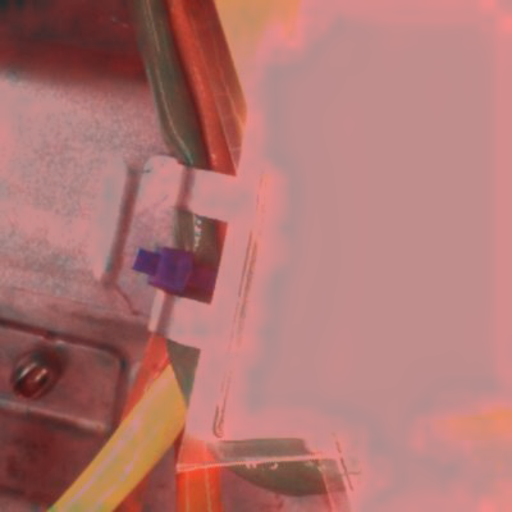
\includegraphics[width=0.26\textwidth]{figures/engine_wiring_0003_anomaly.png} &
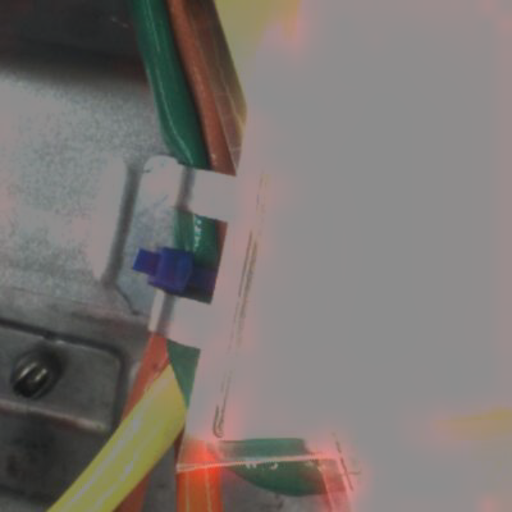
\includegraphics[width=0.26\textwidth]{figures/engine_wiring_0003_gradcam.png} &
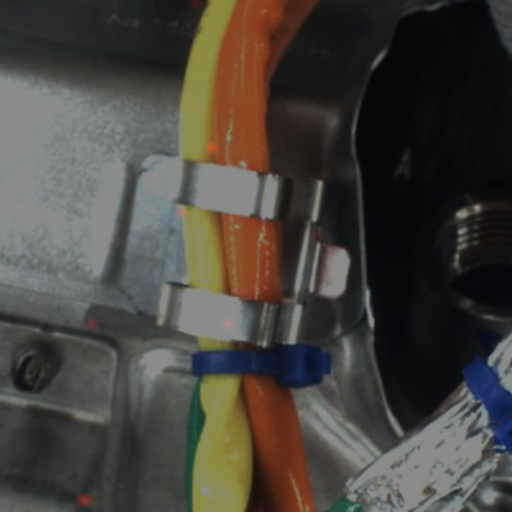
\includegraphics[width=0.26\textwidth]{figures/engine_wiring_0003_shap.png} \\
\texttt{pipe\_clip} &
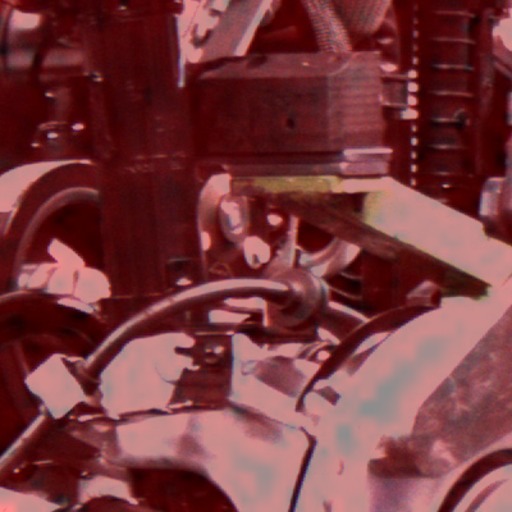
\includegraphics[width=0.26\textwidth]{figures/pipe_clip_0003_anomaly.png} &
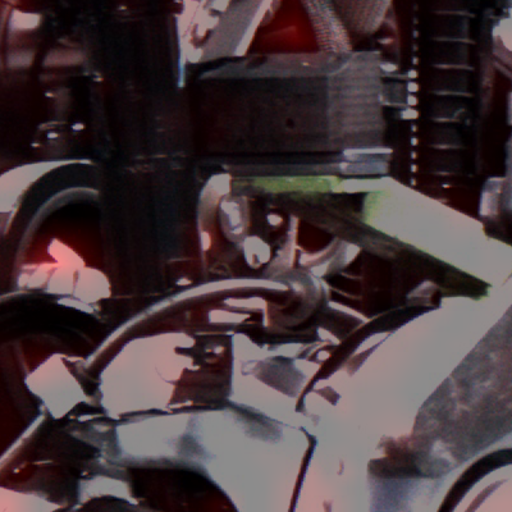
\includegraphics[width=0.26\textwidth]{figures/pipe_clip_0003_gradcam.png} &
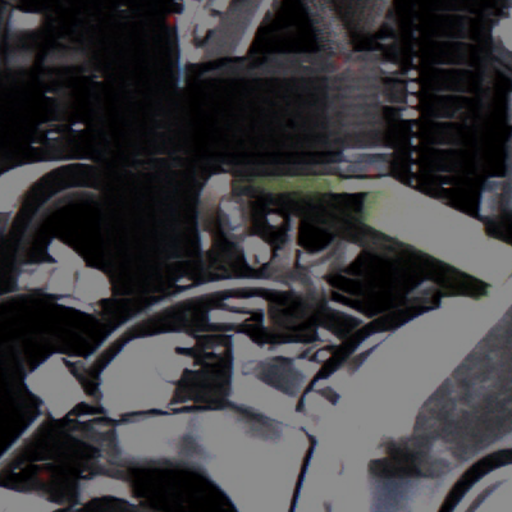
\includegraphics[width=0.26\textwidth]{figures/pipe_clip_0003_shap.png} \\
\end{tabular}
\caption{Interpretability views for two categories. Anomaly heatmaps show patch-distance scores, Grad-CAM highlights salient features, and SHAP shows patch attributions for the anomaly score.}
\label{fig:interpretability-kcenter}
\end{figure*}
\FloatBarrier
\begin{figure}[htbp]
    \centering
    
    % Top row
    \begin{subfigure}[b]{0.45\textwidth}
        \centering
        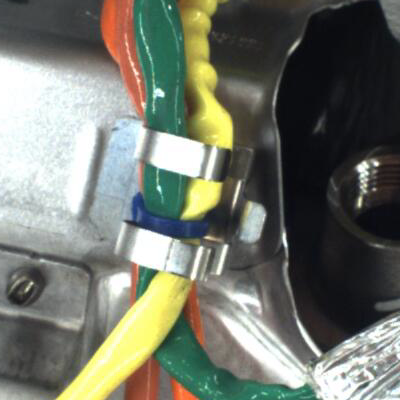
\includegraphics[width=\textwidth]{figures/good.png}
        \caption{Quality engine wiring}
    \end{subfigure}
    \hfill
    \begin{subfigure}[b]{0.45\textwidth}
        \centering
        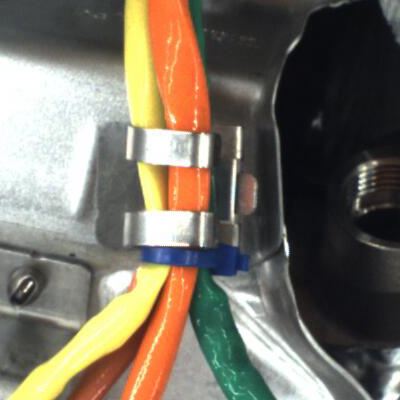
\includegraphics[width=\textwidth]{figures/bad.png}
        \caption{Defective engine wiring (blue hoop out of place)}
    \end{subfigure}
    
    \vspace{0.5cm}
    
    % Bottom row
    \begin{subfigure}[b]{0.45\textwidth}
        \centering
        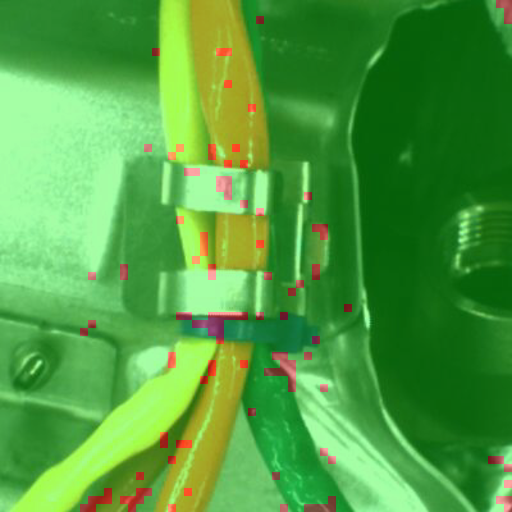
\includegraphics[width=\textwidth]{figures/0000_patch_quality.png}
        \caption{Anomaly heatmap overlay}
    \end{subfigure}
    \hfill
    \begin{subfigure}[b]{0.45\textwidth}
        \centering
        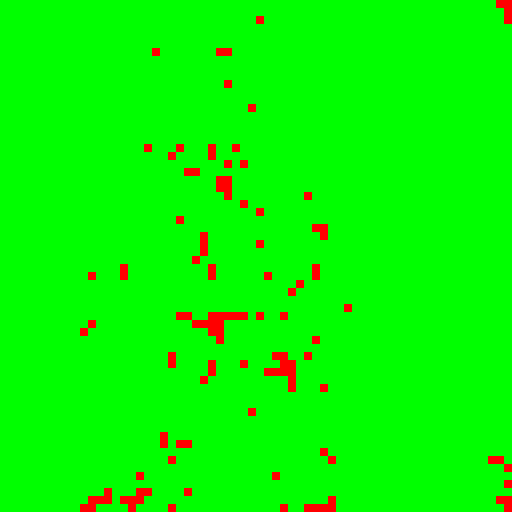
\includegraphics[width=\textwidth]{figures/0000_patch_quality_overlay_only.png}
        \caption{Anomaly heatmap}
    \end{subfigure}
    
    \caption{Simplified anomaly heatmap view}
    \label{fig:four_grid}
\end{figure}

\FloatBarrier



\subsection{Robustness}

 We implemented robustness by injecting controlled corruptions and Gaussian noise during training, then hardening the feature bank and scoring pipeline with norm/cosine filters and optional score clipping. On the federated side, uploads are chunked and audited with norm/cosine sanity checks and outlier handling, and aggregation can be made robust via median/trimmed‑mean client filtering. These options are exposed as CLI flags so we can sweep low/medium/high noise regimes and compare how performance degrades or stabilizes under corruption.

 \paragraph*{Justification}

Using an additive perturbation $\mathcal{N}(0, \sigma_r^2)$ applied per pixel per channel, robustness experiments introduce Gaussian noise directly into the input image tensor following normalization.  

Three different noise levels are assessed: low noise ($\sigma_r = 0.05$), medium noise ($\sigma_r = 0.10$), and high noise ($\sigma_r = 0.20$), which correspond to approximately $5\%$, $10\%$, and $20\%$ of the normalized pixel range. 
These values, which are displayed as the \texttt{--gaussian-noise-std} flag in the training configuration, were selected to cover the range from imperceptible perturbation to visually degraded input. 
In order to simulate production-line variability in illumination and focus, corruption augmentation during training uses \texttt{corruption\_prob} $= 0.5$ and \texttt{corruption\_strength} $= 0.2$, applying random color jitter, autocontrast, sharpness adjustment, and Gaussian blur with probability $0.5$ per image—a standard multi-corruption protocol.

 \begin{figure}[htbp]
    \centering
    
\includegraphics[width=\textwidth]{figures/comparison006.png}
    \caption{Comprehensive performance comparison showing: (top-left) image-level AUROC, (top-right) pixel-level AUROC,  (bottom) average metrics across all categories.}
    \label{fig:comparison006}
\end{figure}
\FloatBarrier

\begin{figure}[htbp]
    \centering
    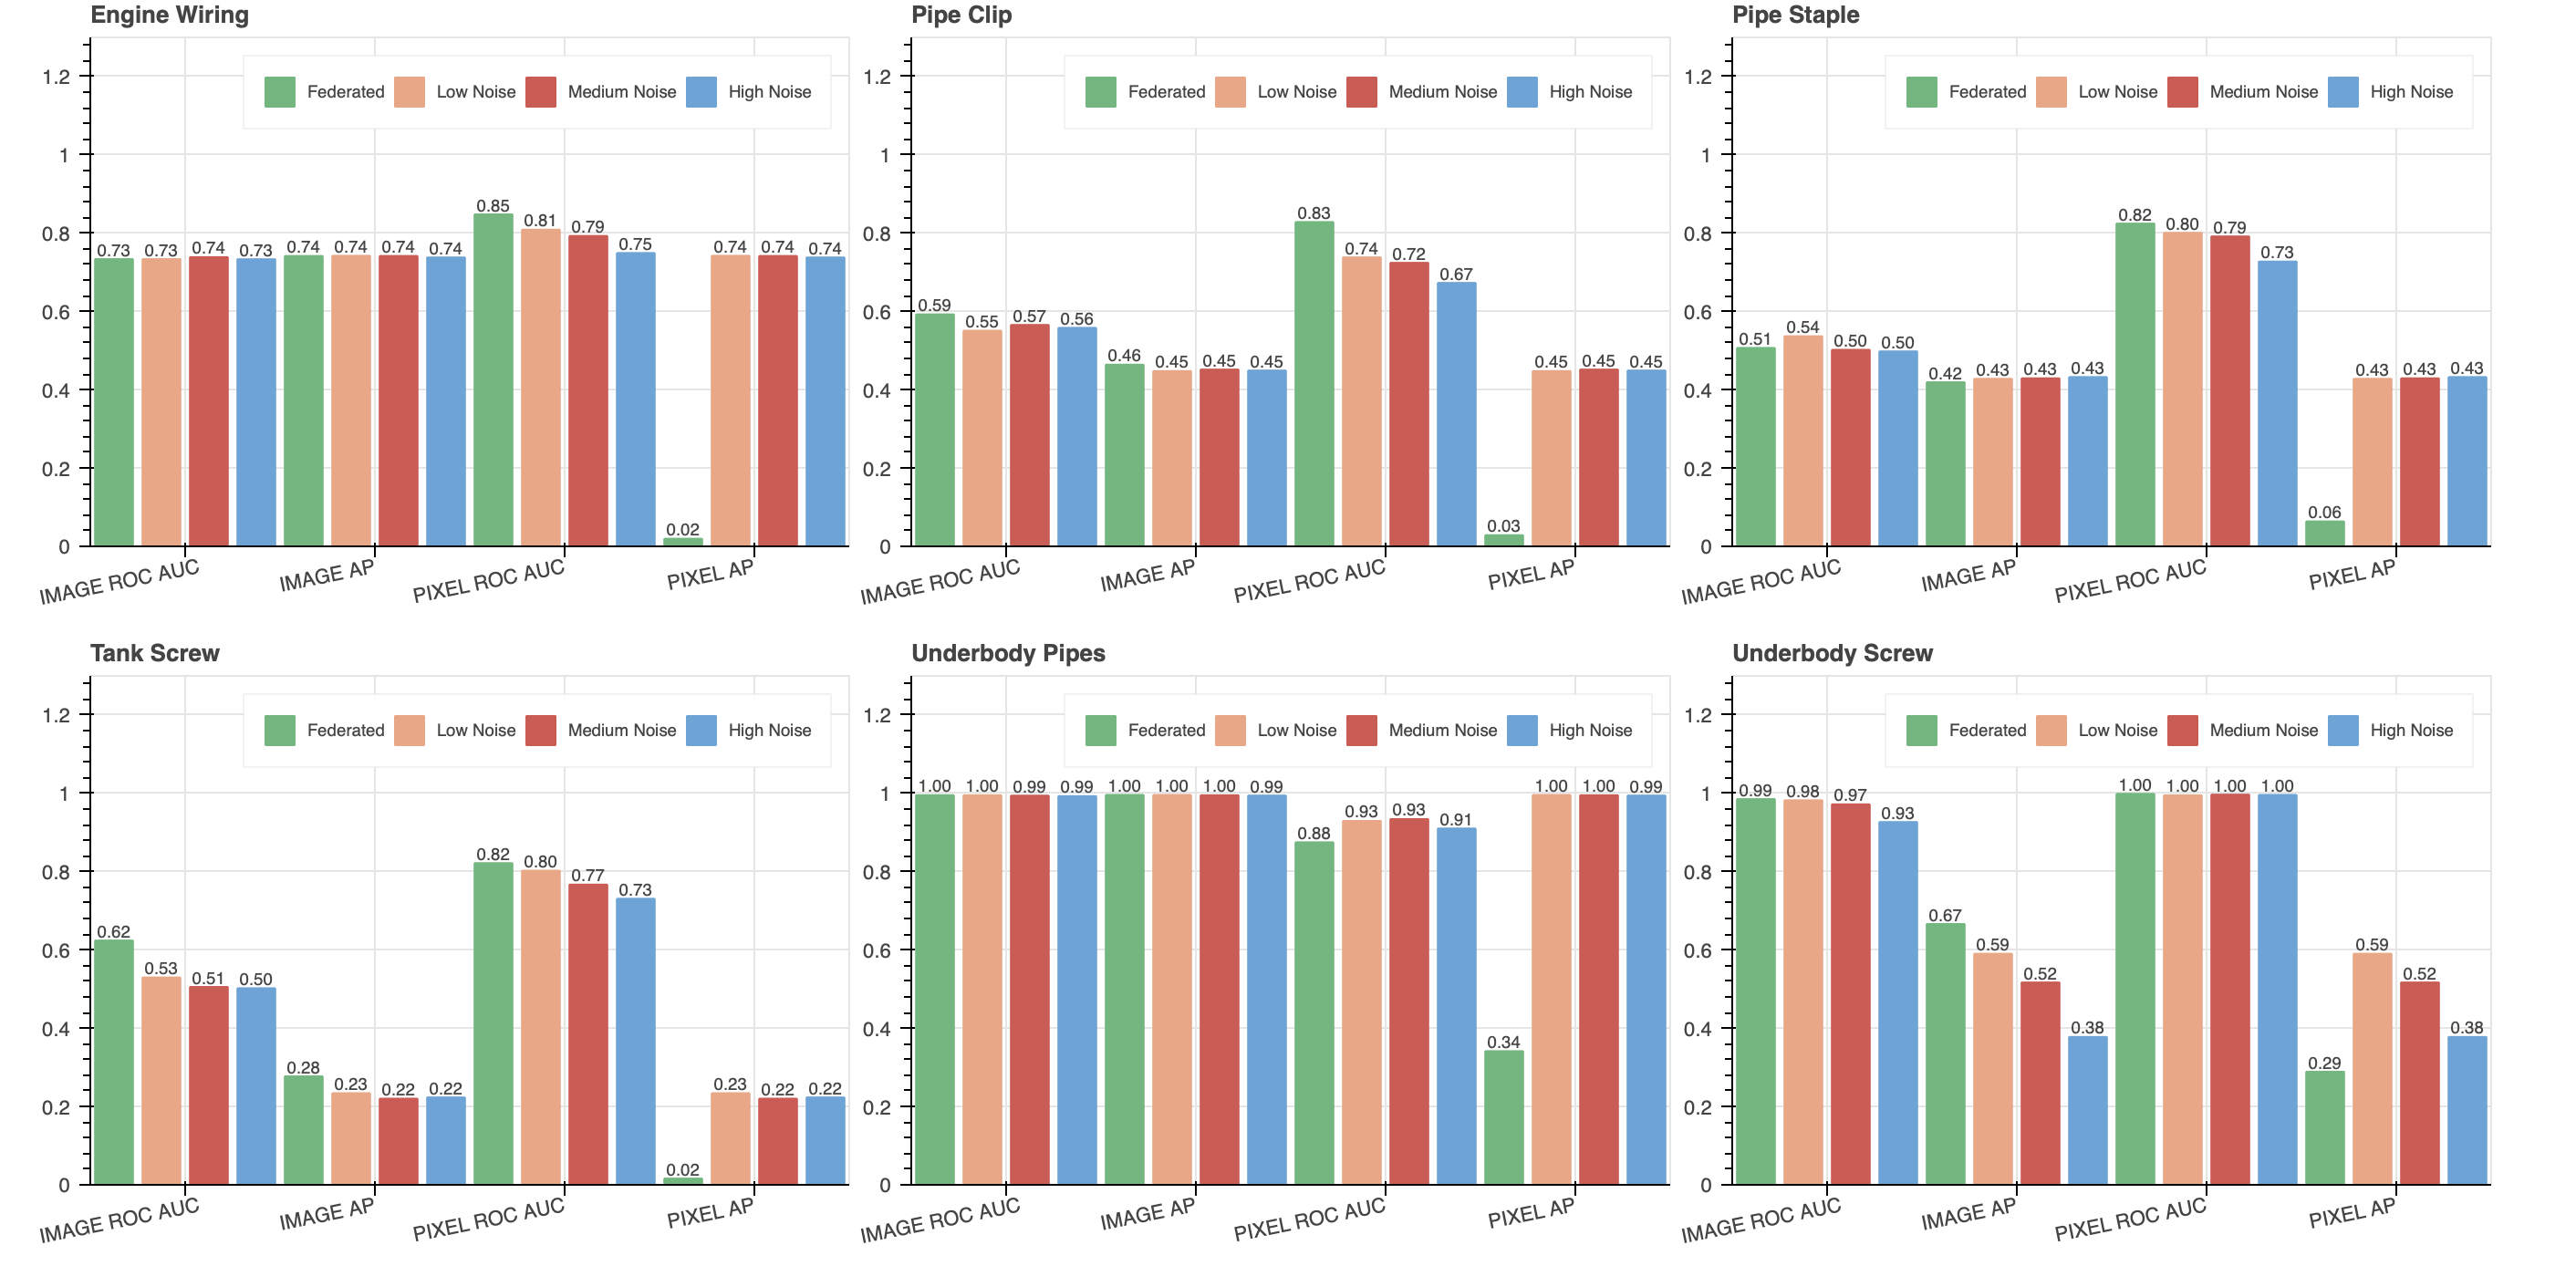
\includegraphics[width=\textwidth]{figures/detailed-comparison006.png}
    \caption{Detailed per-category comparison of all four evaluation metrics (Image AUROC, Pixel AUROC, Image AP, Pixel AP) between centralized and federated approaches.}
    \label{fig:detailed_comparison006}
\end{figure}

With low-noise corruption, the image-level ROC AUC decreases marginally across all categories ($\text{avg.}\ 0.74 \to 0.72$). This shows that the k-center memory bank has enough coverage to handle a small shift in distribution at test time. With medium noise, the performance drops by about $0.01$–$0.02$ per category, but it stays in the same range. High noise is the first level where we can see real degradation: at the image level, \texttt{tank\_screw} drops from $0.62$ to $0.50$ and \texttt{pipe\_clip} drops from $0.59$ to $0.56$. The pixel ROC AUC also drops more broadly ($\text{avg.}\ 0.87 \to 0.81$). 
The underbody categories remain robust even under high noise levels (image AUC $\geq 0.93$ for \texttt{underbody\_pipes}), which can be explained by their larger training sets covering more memory banks. Pixel AP is more sensitive than ROC AUC at all noise levels. The only exception is \texttt{underbody\_screw}, which keeps a strong pixel AP ($0.38$ at high noise vs. $0.29$ at baseline). Overall, the federated pipeline is fairly strong against moderate input corruption. As noise increases, localization metrics get worse faster than image-level discrimination.

\section{Ablation study}

The strategy we adopted for our study was to start with a base model and progressively add enhancements on top it as shown in Figure \ref{fig:ablation-strategy} . In this respect, after we identified the base model as PatchCore, we implemented the training pipeline in a centralized fashion and we ran two ablations where we varied the coreset selection algorithm, from Random to K-Center. Then we implemented the federated learning scenario and we distributed the data between three clients in a non-IID fashion. The first two ablations also varied the coreset selection algorithm.

\begin{figure}[htbp]
    \centering
    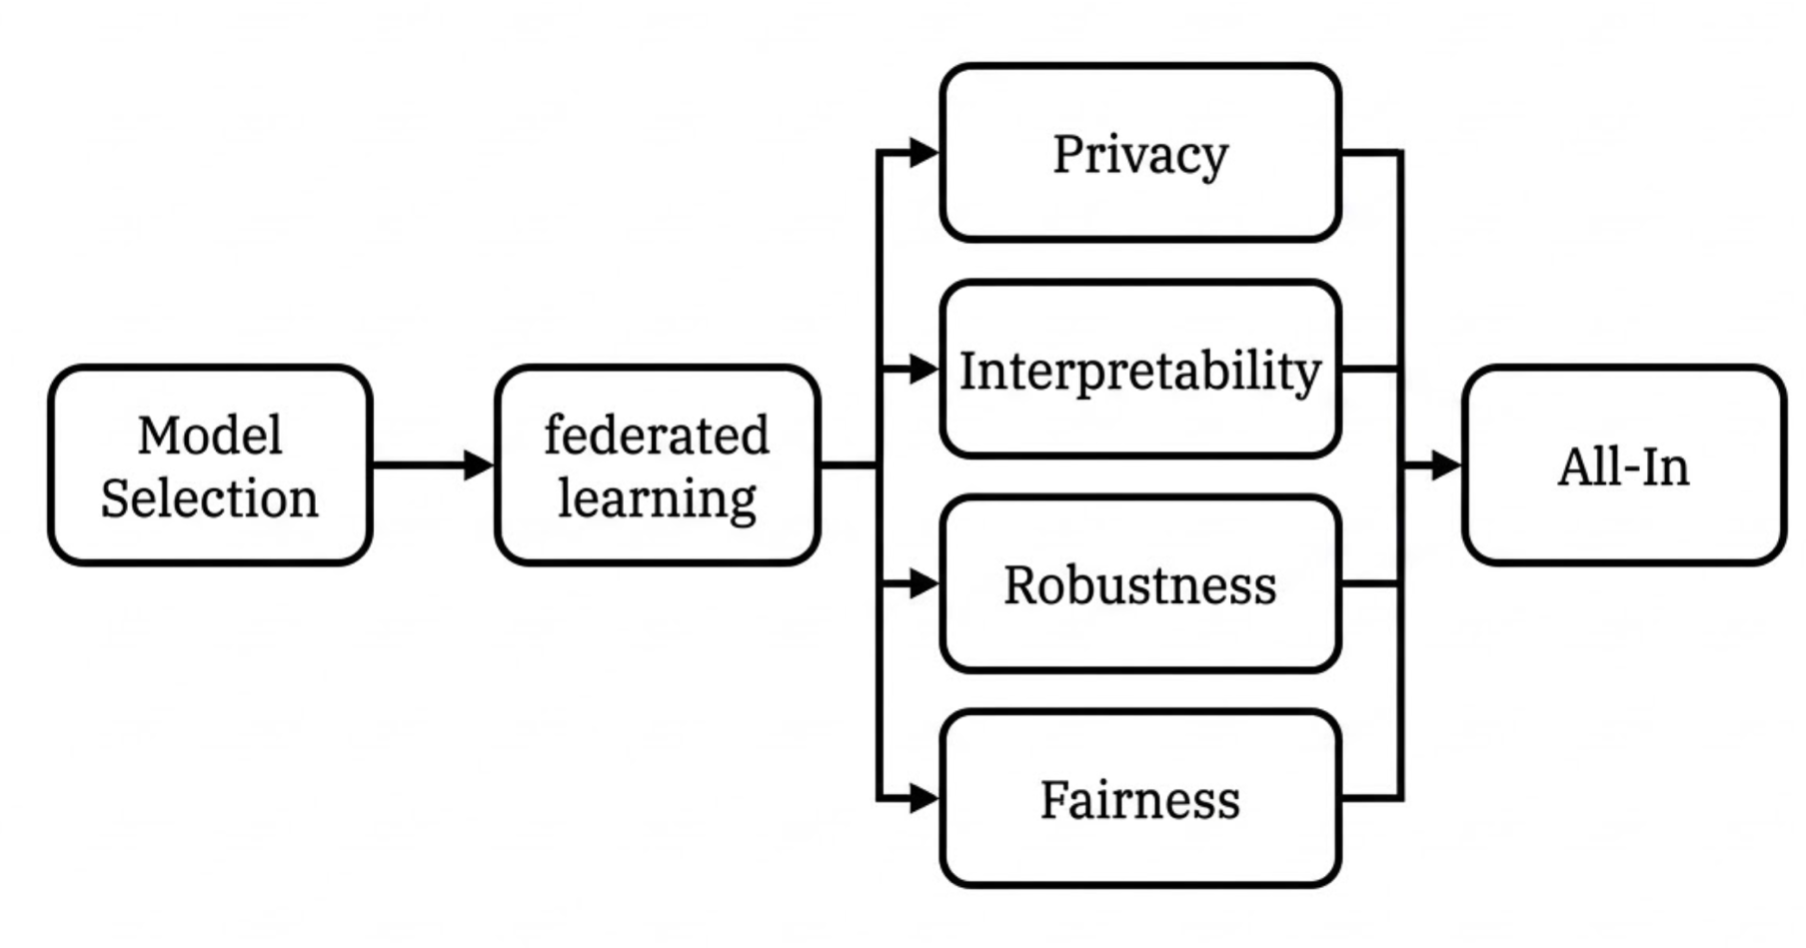
\includegraphics[width=\textwidth]{figures/ablation-strategy.png}
    \caption{Ablation strategy}
    \label{fig:ablation-strategy}
\end{figure}

All subsequent ablations continued with the federated learning approach with the K-Center coreset selection algorithm. For the next two ablations we implemented first differential privacy, then Renyi DP. The trainings were ran with only one of these enabled. Continuing with trustworthiness inducing features like fairness, noise injection along with robustness enhancers with various levels of noise and interpretability. In the results table interpretability is not tracked explicitly because it has no effect on model performance. The last ablation was ran with multiple features enabled - Renyi DP plus medium noise injection for robustness enhancer.


\begin{table*}[htbp]
\centering
\adjustbox{max width=\textwidth}{%
\begin{tabular}{l cccccc c}
\toprule
\textbf{Ablation}
  & \textbf{eng\_wiring}
  & \textbf{pipe\_clip}
  & \textbf{pipe\_staple}
  & \textbf{tank\_screw}
  & \textbf{und\_pipes}
  & \textbf{und\_screw}
  & \textbf{Avg} \\
\midrule
CenRandom        & 0.55 & 0.51 & 0.59 & 0.47 & 0.83 & 0.61 & 0.59 \\
CenK-Center      & 0.66 & 0.52 & 0.47 & 0.57 & 0.95 & 0.95 & 0.69 \\
FedRandom        & 0.63  & 0.53  & 0.61  & 0.44  & 0.97  & 0.64  & 0.64 \\
FedK-Center      & 0.73 & 0.59 & 0.51 & 0.62 & 1.00 & 0.99 & 0.74 \\
FedKC+DP         & 0.55 & 0.50 & 0.50 & 0.45 & 0.80 & 0.60 & 0.58 \\
FedKC+RDP        & 0.56 & 0.56 & 0.59 & 0.42 & 0.79 & 0.51 & 0.57 \\
Fairness         & 0.61 & 0.54 & 0.52 & 0.46 & 0.97 & 0.65 & 0.62 \\
FedKC+LowNoise   & 0.73 & 0.55 & 0.54 & 0.53 & 1.00 & 0.98 & 0.72 \\
FedKC+MedNoise   & 0.74 & 0.57 & 0.50 & 0.51 & 0.99 & 0.97 & 0.71 \\
FedKC+HiNoise    & 0.75 & 0.56 & 0.50 & 0.50 & 0.99 & 0.93 & 0.70 \\
FedKC+RDP+Med    & 0.55  & 0.50  & 0.61  & 0.41  & 0.75  & 0.72  & 0.59 \\
\bottomrule
\end{tabular}%
}
\caption{Image-level ROC AUC across all ablations.}
\label{tab:full_ablation_auroc}
\end{table*}

\begin{table*}[htbp]
\centering
\adjustbox{max width=\textwidth}{%
\begin{tabular}{l cccccc c}
\toprule
\textbf{Ablation}
  & \textbf{eng\_wiring}
  & \textbf{pipe\_clip}
  & \textbf{pipe\_staple}
  & \textbf{tank\_screw}
  & \textbf{und\_pipes}
  & \textbf{und\_screw}
  & \textbf{Avg} \\
\midrule
CenRandom        & 0.86 & 0.81 & 0.79 & 0.82 & 0.88 & 0.99 & 0.86 \\
CenK-Center      & 0.84 & 0.82 & 0.83 & 0.78 & 0.86 & 0.99 & 0.85 \\
FedRandom        & 0.86  & 0.81  & 0.86  & 0.82  & 0.87  & 0.98  & 0.85  \\
FedK-Center      & 0.85 & 0.83 & 0.82 & 0.82 & 0.88 & 1.00 & 0.87 \\
FedKC+DP         & 0.65 & 0.62 & 0.52 & 0.62 & 0.64 & 0.85 & 0.65 \\
FedKC+RDP        & 0.67 & 0.57 & 0.54 & 0.50 & 0.65 & 0.85 & 0.63 \\
Fairness         & 0.86 & 0.81 & 0.80 & 0.82 & 0.88 & 0.98 & 0.86 \\
FedKC+LowNoise   & 0.81 & 0.74 & 0.80 & 0.80 & 0.93 & 1.00 & 0.85 \\
FedKC+MedNoise   & 0.81 & 0.72 & 0.79 & 0.77 & 0.93 & 1.00 & 0.84 \\
FedKC+HiNoise    & 0.79 & 0.67 & 0.73 & 0.73 & 0.91 & 1.00 & 0.81 \\
FedKC+RDP+Med    & 0.59  & 0.54  & 0.44  & 0.60  & 0.71  & 0.83  & 0.61  \\
\bottomrule
\end{tabular}%
}
\caption{Pixel-level ROC AUC across all ablations.}
\label{tab:full_ablation_pixel_auroc}
\end{table*}

\FloatBarrier

We track detailed ablation results in Tables \ref{tab:full_ablation_auroc} and \ref{tab:full_ablation_pixel_auroc}, more specifically image level and pixel level AUROC scores for each label and average across all labels. From these detailed results we distill the following key findings, first at image level:
\begin{itemize}
	\item K-Center consistently outperforms random coreset selection (+10\% for both centralized and federated approaches)
	\item Federated learning outperforms centralized learning (+5\% across both coreset selection strategies)
	\item Performance is not consistent among classes, underbody pipes and screws outperforming the other classes by a rather large margin
	\item Privacy is costly (-16\%) and Renyi DP doesn't help, on the contrary on average it brings -1\% penalty
	\item Noise robustness degrades linearly with the noise increse
\end{itemize}

However, at pixel level:
\begin{itemize}
	\item Unlike the image level scores, here random and K-Center coreset sampling score similarly, just like centralized and federated approaches
	\item Fairness is essentially free at pixel level
	\item DP affects in a higher degree the model performance as compared to image level scores (22\% vs 16\%)
	\item Pixel level scores show higher sensitivity to noise than image level scores
\end{itemize}

To conclude, we see that underbody labels perform better than the other labels, and that trustworthy AI extensions primarily erode performance on the labels that already perform poorly while the underbody labels remain resilient.

\section{Experimental Results on Additional Datasets}

In this section, we present the experimental results obtained on the three additional industrial datasets introduced previously: \textit{XFK3}, \textit{Pompe}, and \textit{Radiateur}.
All experiments follow the same anomaly detection protocol, using PatchCore with a k-center coreset strategy in a federated sequential setup.

Since these datasets do not provide pixel-level segmentation masks for defective regions, evaluation is primarily conducted at the \textbf{image level}. Pixel-level metrics are reported for completeness but are not considered meaningful in this context.

\subsection{Evaluation Metrics}

We report the following metrics:
\begin{itemize}
    \item \textbf{Image-level ROC AUC}: measures the ability of the model to distinguish between OK and KO samples.
    \item \textbf{Image-level Average Precision (AP)}: evaluates ranking quality under class imbalance.
    \item \textbf{Pixel-level ROC AUC and AP}: reported as NaN due to the absence of ground-truth segmentation masks.
\end{itemize}

\subsection{XFK3 Results}

The XFK3 dataset exhibits a very low number of defective samples in the test split, making it a challenging yet realistic anomaly detection scenario.

Despite this strong imbalance, the model achieves perfect discrimination between OK and KO samples.

\begin{table}[htbp]
    \centering
    \begin{tabular}{l r}
        \hline
        \textbf{Metric} & \textbf{Value} \\
        \hline
        Image ROC AUC & 1.000 \\
        Image AP & 1.000 \\
        Pixel AP & 1.000 \\
        Total Test Images & 136 \\
        \hline
    \end{tabular}
    \caption{Performance metrics for the XFK3 dataset.}
    \label{tab:xfk3_results}
\end{table}

These results indicate that the learned representation captures the nominal appearance of the component with high precision, enabling reliable anomaly detection even with extremely limited defective data.

\subsection{Pompe Results}

The Pompe dataset presents a more balanced yet still realistic distribution of OK and KO samples.
The model achieves strong image-level performance, demonstrating robustness to variations in defect appearance.

\begin{table}[htbp]
    \centering
    \begin{tabular}{l r}
        \hline
        \textbf{Metric} & \textbf{Value} \\
        \hline
        Image ROC AUC & 0.921 \\
        Image AP & 0.639 \\
        Pixel AP & 0.639 \\
        Total Test Images & 33 \\
        \hline
    \end{tabular}
    \caption{Performance metrics for the Pompe dataset.}
    \label{tab:pompe_results}
\end{table}

The high ROC AUC value indicates reliable separation between normal and defective samples, while the lower AP reflects the limited number of positive (KO) examples in the test set.

\subsection{Radiateur Results}

The Radiateur dataset is characterized by subtle defects and visually complex assemblies, making anomaly detection more challenging.

\begin{table}[htbp]
    \centering
    \begin{tabular}{l r}
        \hline
        \textbf{Metric} & \textbf{Value} \\
        \hline
        Image ROC AUC & 0.706 \\
        Image AP & 0.596 \\
        Pixel AP & 0.596 \\
        Total Test Images & 38 \\
        \hline
    \end{tabular}
    \caption{Performance metrics for the Radiateur dataset.}
    \label{tab:radiateur_results}
\end{table}

Although performance is lower compared to XFK3 and Pompe, the results remain well above random chance, highlighting the difficulty of detecting fine-grained structural anomalies in this dataset.

\subsection{Discussion}

Across all three datasets, the proposed approach demonstrates strong image-level anomaly detection performance, even in the presence of:
\begin{itemize}
    \item severe class imbalance,
    \item heterogeneous industrial components,
    \item absence of pixel-level annotations.
\end{itemize}

The NaN values observed for pixel-level ROC AUC are expected and stem from the lack of ground-truth segmentation masks. Consequently, image-level metrics provide the most reliable evaluation signal for these datasets.

\begin{figure}[htbp]
    \centering
    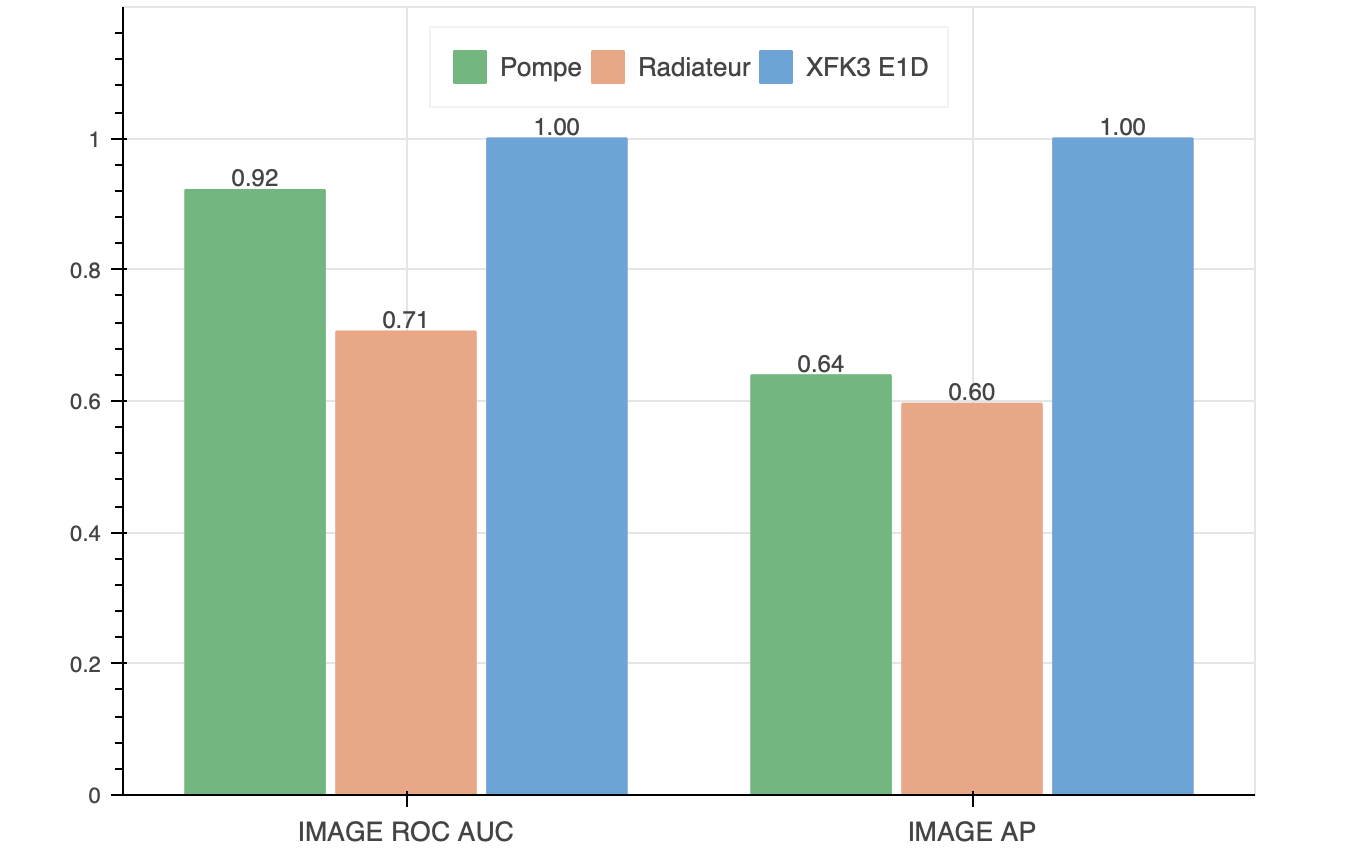
\includegraphics[width=\textwidth]{figures/extra-comparison.png}
    \caption{Comparison for image level scores across the 3 categories}
    \label{fig:extra-comparison}
\end{figure}

Overall, these results validate the applicability of federated PatchCore to real-world industrial inspection scenarios involving diverse components and limited defect annotations.

\section{Conclusions}
We presented an industrial anomaly detection pipeline built on PatchCore and evaluated it on the AutoVI dataset under both centralized and federated settings. The results show that strong performance can be achieved with coreset-based memory banks while keeping inference efficient, and that federated training is viable under non‑IID splits when aggregation and sampling are handled carefully. We also examined trustworthy‑AI extensions: differential privacy for memory‑bank sharing, robustness via corruption and feature filtering, and interpretability through anomaly heatmaps, Grad‑CAM, and SHAP. These additions make the system more transparent and resilient, but they introduce measurable trade‑offs in detection performance, especially under higher noise and privacy budgets. Finally, qualitative tests on extra datasets suggest that the approach generalizes reasonably but remains sensitive to domain shifts.

\begin{figure}[htbp]
    \centering
    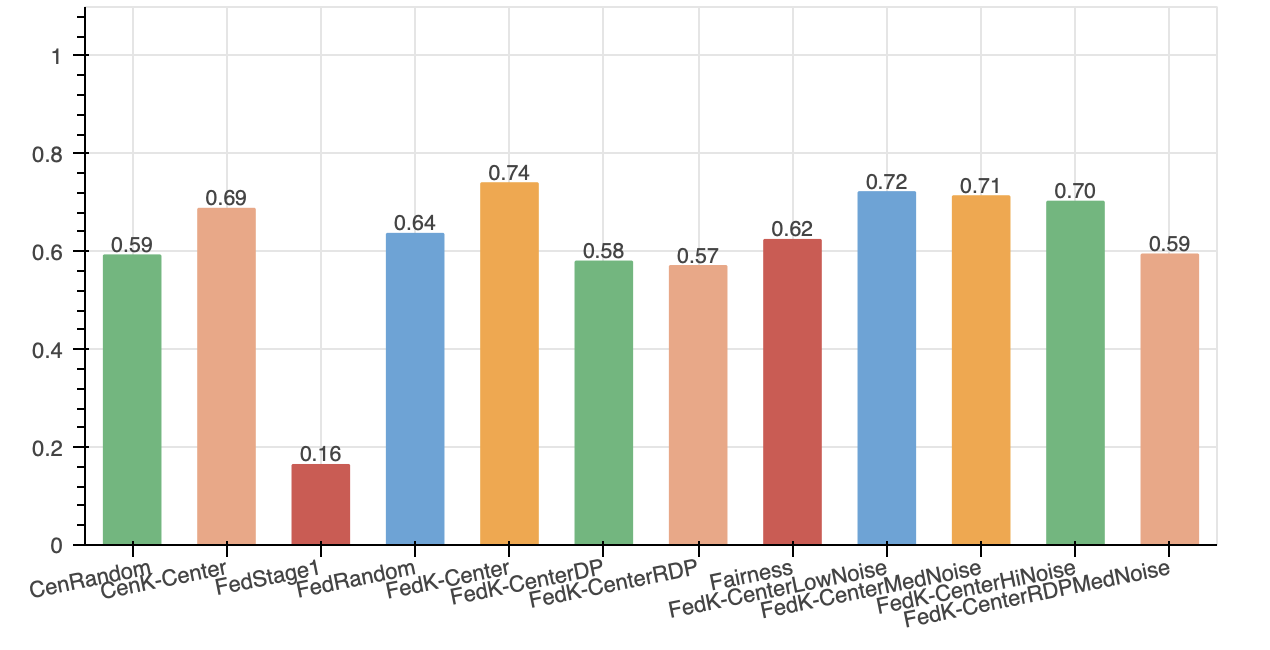
\includegraphics[width=\textwidth]{figures/fullcomparison.png}
    \caption{Comparison for AUROC image level scores for all ablations}
    \label{fig:extra-comparison}
\end{figure}

\appendix
\section{Repository Description}

The complete implementation and experimental setup for this project is available at: \url{https://github.com/icordos/automotive-anomaly-detection}

\subsection{Directory Structure}

The repository is organized as follows:

\begin{description}
    \item[\texttt{src/}] Main source code directory containing all implementations:
    \begin{itemize}
        \item \texttt{centralized/}: Centralized PatchCore training and evaluation pipeline
        \item \texttt{federated/}: Final federated learning implementation with sequential client-server communication
        \item \texttt{federated-stage1/}: Initial federated learning prototype
        \item \texttt{data/}: Dataset handling utilities and download scripts
        \item \texttt{scripts\_dp\_fairness/}: Experimental scripts for differential privacy and fairness-aware coreset selection
        \item \texttt{scripts\_no\_dp\_fairness/}: Baseline experimental scripts
    \end{itemize}

    \item[\texttt{results/}] Experimental results and artifacts from different runs:
    \begin{itemize}
        \item Timestamped directories containing client metrics, server outputs, and logs
        \item Supports both centralized and federated configurations with various privacy settings (DP, fairness)
        \item Includes robustness testing results with different corruption levels
    \end{itemize}

    \item[\texttt{paper/}] LaTeX source code for the research paper:
    \begin{itemize}
        \item \texttt{report-1.tex}: Main paper document
        \item \texttt{neurips\_2024.sty}: NeurIPS 2024 conference style
        \item \texttt{references.bib}: Bibliography entries
        \item \texttt{interpretability/}: Visualization outputs (Grad-CAM, SHAP, anomaly overlays)
    \end{itemize}

    \item[\texttt{docs/}] Documentation:
    \begin{itemize}
        \item \texttt{federated\_guide.md}: Comprehensive guide for running federated experiments
        \item \texttt{croissant.json}: Croissant metadata for dataset description
        \item \texttt{datasheet}: Datasheet documentation following Gebru et al. framework
    \end{itemize}
\end{description}

\subsection{Key Files and Usage}

\begin{description}
    \item[\texttt{requirements.txt}] Python package dependencies (flwr, torch, torchvision, scikit-learn, etc.)

    \item[\texttt{start-server.sh}, \texttt{start-client-*.sh}] Bash scripts for launching federated learning experiments

    \item[\texttt{start-centralized.sh}] Script for running centralized training baseline
\end{description}

\subsection{Running Experiments}

Setup requirements:
\begin{enumerate}
    \item Install Python dependencies: \texttt{pip install -r requirements.txt}
    \item Download the AutoVI dataset: \texttt{./src/data/download\_datasets.sh --data-root data}
\end{enumerate}

To run centralized baseline:
\begin{verbatim}
./src/centralized/patchcore_training.py \
  --dataset-root data/raw \
  --categories engine_wiring pipe_clip
\end{verbatim}

To run federated experiments, start the server first, then launch multiple clients. Refer to \texttt{docs/federated\_guide.md} for detailed configuration options including differential privacy and fairness-aware coreset selection.

\section{Preprocessing Pipeline}
The data is hosted on Zenodo and is described in a croissant file provided by Renault. For each of the six categories the croissant metadata points to a zip archive. We have used the exact structure provided by Renault and the only preprocessing that we did was to unzip the archives.
\\
The dataset is structured per category as follows:
\begin{itemize}
	\item \textbf{train}: the train folder contains only "good" images for each category
	\item \textbf{test}: the test folder contains one subdirectory per defect type (e.g. missing, contamination, etc) plus a good folder
	\item \textbf{ground\_truth}: for every anomalous test image, pixel annotations are stored at ground\_truth/<defect-name>/<image-stem>/0000.png
	\item \textbf{defects\_config.json}: metadata about defect types.
	\item \textbf{defect\_example.png}: visualization of defects
\end{itemize}


\bibliographystyle{plainnat}
\bibliography{references}

\end{document}
